%% ---------------------------------------------------------------------------
%% Memoria de Proyecto Fin de Master - Tecnun / MADI
%% Compilar:  ./compilar.sh        (o make)
%% Citas IEEE: \cite{clave} -> [1]  |  bibliografia: bib/referencias.bib
%% ---------------------------------------------------------------------------
\documentclass[11pt,a4paper,twoside,openright]{report}

\usepackage{tecnun-tfm}

% --- Datos de la memoria -----------------------------------------------------
\tfmtipo{Proyecto Fin de M\'aster}
\tfmmaster{AN\'ALISIS DE DATOS EN INGENIER\'IA}
\tfmtitulo{Comparaci\'on de codificadores visuales en Diffusion Policy:
           protocolo con prueba disjunta, rendimiento y coste en Push-T}
\tfmtitulocorto{Codificadores visuales en Diffusion Policy}
\tfmautor{Moises Britez}
\tfmdirector{Diego Borro}                    % dejar vacio si no procede
\logotecnun{img/logo.png}
\tfmlugar{Donostia-San Sebasti\'an}
\tfmfecha{septiembre de 2026}

\begin{document}

% ============================ PRELIMINARES ==================================
% Orden fijado por normas_redaccion.md: portada, primera hoja, agradecimientos,
% indice de contenidos, indice de figuras, indice de tablas, resumen, abstract.
\portadatfm

\pagenumbering{roman}
% Primera hoja exigida por las normas de redaccion. La plantilla oficial se
% distribuye en Word con el logo de Tecnun incrustado en EPS. Aqui se reproduce
% su contenido como hoja de identificacion; sustituir por la version oficial si
% el centro la exige literal.
\thispagestyle{empty}
\begin{center}
  \vspace*{2cm}
  {\fontsize{14}{18}\selectfont\bfseries \tfmtituloactual\par}
  \vspace{3cm}

  {\normalsize
   Memoria presentada por \tfmautoractual\ para la obtenci\'on del t\'itulo de
   M\'aster Universitario en \MakeLowercase{\tfmmasteractual}.\par}
  \vspace{2cm}

  {\normalsize \tfmdirectoractual\par}
  \vspace{3.5cm}

  \begin{minipage}{0.42\textwidth}\centering
    \rule{0.8\textwidth}{0.4pt}\\
    \small Fdo.: \tfmautoractual
  \end{minipage}\hfill
  \begin{minipage}{0.42\textwidth}\centering
    \rule{0.8\textwidth}{0.4pt}\\
    \small Fdo.: el director
  \end{minipage}

  \vfill
  {\normalsize \tfmlugaractual, \tfmfechaactual\par}
\end{center}
\cleardoublepage


\preliminar{Agradecimientos}

[Texto de agradecimientos. Esta pagina es opcional y no lleva numeracion de
capitulo. Se redacta en primera persona, unica excepcion al estilo impersonal
del resto de la memoria.]


\tableofcontents
\cleardoublepage
\listoffigures
\cleardoublepage
\listoftables
\cleardoublepage

\preliminar{Resumen del proyecto}

\textit{Diffusion Policy} genera acciones de manipulaci\'on rob\'otica mediante un proceso
de difusi\'on condicionado por la observaci\'on. Su variante visuomotora encadena un
codificador visual y una red generativa, de modo que la representaci\'on de la imagen
delimita la informaci\'on disponible para el control. La investigaci\'on posterior ha
modificado sobre todo el bloque generativo, mientras que la elecci\'on del codificador y de
su estrategia de entrenamiento sigue sin resolverse cuando solo se dispone de un conjunto
reducido de demostraciones.

Este trabajo eval\'ua la influencia del codificador visual y de su estrategia de
entrenamiento sobre el rendimiento de una \textit{Diffusion Policy} en la tarea Push-T. Con
ese fin se implementan cinco variantes del codificador dentro de la misma pol\'itica: una
ResNet-18 entrenada desde cero, la misma red preentrenada sobre ImageNet en versiones
congelada y con ajuste fino, y dos transformadores de visi\'on congelados, DINOv2 ViT-S/14
y CLIP ViT-B/16. Todas entregan un vector de \num{512} componentes y comparten red
generativa, hiperpar\'ametros, datos y protocolo de evaluaci\'on, de manera que la \'unica
variable manipulada es el codificador. El ajuste emplea \num{206} demostraciones
teleoperadas y un presupuesto m\'aximo de \num{500} \'epocas con parada anticipada. La
evaluaci\'on mide la puntuaci\'on media de cobertura sobre \num{50} episodios generados
con semillas reservadas, junto con el tiempo de c\'omputo consumido.

Los resultados corresponden a las tres variantes convolucionales completadas, ya que las
dos basadas en transformador siguen en ejecuci\'on. La l\'inea base entrenada desde cero
alcanza una puntuaci\'on de \num{0.864}, frente a \num{0.668} de la variante congelada y
\num{0.648} de la ajustada, ca\'idas del \SI{23}{\percent} y del \SI{25}{\percent} cuyos
intervalos de confianza excluyen el cero. El
preentrenamiento tampoco compensa en coste: cada \'epoca de la l\'inea base ocupa
\SI{1.5}{\minute}, frente a \SI{5.3}{\minute} y \SI{14.7}{\minute} de las variantes
preentrenadas, y las tres ejecuciones suman casi \num{200} horas de procesamiento
gr\'afico. Ese sobrecoste se atribuye a la resoluci\'on de entrada y no al n\'umero de
par\'ametros entrenables, que apenas var\'ia entre variantes.

Se concluye que, en Push-T y con pocas demostraciones, el preentrenamiento supervisado
sobre im\'agenes naturales degrada el rendimiento y encarece el entrenamiento. La ventaja
de la l\'inea base debe atribuirse al codificador junto con su cadena de preprocesado,
puesto que ambos var\'ian de forma conjunta.

\vspace{1em}
\noindent\textbf{Palabras clave:} aprendizaje por imitaci\'on, modelos de difusi\'on,
codificador visual, transferencia de aprendizaje, manipulaci\'on rob\'otica.

\preliminar{Abstract}

\begin{otherlanguage}{english}
% El entorno abre grupo: la marca decimal inglesa no escapa de este apartado.
\sisetup{output-decimal-marker={.}}

\textit{Diffusion Policy} generates robotic manipulation actions through a diffusion
process conditioned on the observation. Its visuomotor variant chains a visual encoder and
a generative network, so the image representation bounds the information available for
control. Subsequent research has mostly modified the generative block, whereas the choice
of encoder and of its training strategy remains unsettled when only a small set of
demonstrations is available.

This work compares five visual blocks integrated as the observation encoder of a single
\textit{Diffusion Policy} on the Push-T task: a ResNet-18 trained from scratch, the same
network pretrained on ImageNet in frozen and fine-tuned versions, and two frozen vision
transformers, DINOv2 ViT-S/14 and CLIP ViT-B/16. All of them output a
\num{512}-component vector and share the generative network, the data, and the evaluation
protocol.
Training uses \num{90} of the \num{206} teleoperated demonstrations, following the
reference implementation, and budgets ranging from \num{200} to
\num{500} epochs, with early stopping. A set of \num{50} episodes generated with held-out
seeds selects the checkpoint of each variant. Performance is then measured once on
\num{200} episodes from a disjoint seed block, under a preregistered protocol, together
with the compute time consumed. Each visual block is trained exactly once, a design
premise adopted in order to cover five configurations within the available compute
budget; the unit of inference is therefore the trained artefact, not the training
strategy.

Each condition is solved with two realisations of the diffusion noise, so that the estimand
integrates both the initial condition and the stochastic sampling of the policy. On that
independent block, the baseline trained from scratch reaches \num{0.887}. The four
pretrained variants score \num{0.642}, \num{0.580}, \num{0.571}, and \num{0.490}. V0
outperforms all of them after the ten pairwise tests are corrected with Holm's procedure,
and this holds regardless of which test is used. Among the pretrained variants, by contrast,
only the weakest separates from the rest under both tests, and the two intermediate ones are
indistinguishable from each other. Each V0 epoch takes \SI{1.6}{\minute}, compared with
\SI{2.3}{\minute} to \SI{14.7}{\minute} for the other variants. The five runs total
\SI{237.1}{\hour}.

A separately preregistered contrast compares that baseline with the checkpoint released by
the authors of the reference implementation. The released model scores \num{0.846}, that is
\num{0.041} lower. With an equivalence margin of \num{0.05} fixed in advance, the data
support the claim that the reproduction does not underperform the reference artefact,
without establishing that it exceeds it by a practically relevant amount. That contrast also
revealed that changing only the noise seed shifts the mean score by \num{0.030}, a magnitude
comparable to the differences separating the pretrained variants from one another, and this
measurement is what prompted duplicating the realisations throughout the final test.

The study concludes that, among the five artefacts evaluated and over the conditions
tested, none of the pretrained visual blocks improves the baseline either in performance
or in cost per epoch. The advantage must be ascribed to the complete visual block
(initial weights, resolution, cropping, and spatial aggregation), which varies jointly,
rather than to pretraining in isolation. With a single training run per variant, the
result does not license extrapolation to the expected behaviour of those strategies upon
retraining.

\vspace{1em}
\noindent\textbf{Keywords:} imitation learning, diffusion models, visual encoder, transfer
learning, robotic manipulation.
\end{otherlanguage}


% ============================== CUERPO ======================================
\cleardoublepage
\pagenumbering{arabic}\setcounter{page}{1}
\tfmpiecompleto

\chapter{Introducci\'on y objetivos}
\label{cap:introduccion}

Este cap\'itulo sit\'ua el trabajo en su \'ambito, delimita el problema que aborda y
enuncia los objetivos que gu\'ian la investigaci\'on. Adem\'as, precisa el alcance del
estudio y describe la organizaci\'on de la memoria.

\section{Contexto y motivaci\'on}
\label{sec:contexto}

La manipulaci\'on rob\'otica requiere generar acciones continuas a partir de
observaciones sensoriales de alta dimensi\'on. El aprendizaje por imitaci\'on aborda esa
dificultad ajustando una pol\'itica sobre demostraciones humanas, sin necesidad de
dise\~nar una funci\'on de recompensa \cite{ross2011dagger}.

Sin embargo, las demostraciones humanas son multimodales. Ante una misma observaci\'on,
un operario puede ejecutar acciones distintas y todas ellas v\'alidas. Los m\'etodos de
clonaci\'on de comportamiento basados en regresi\'on promedian esas alternativas y
producen trayectorias incoherentes \cite{florence2021ibc}.

Para evitar ese promediado, Chi \textit{et al.} \cite{chi2025diffusion} proponen
\textit{Diffusion Policy}, que representa la acci\'on como un proceso de difusi\'on
condicionado por la observaci\'on. El m\'etodo hereda as\'i la capacidad de los modelos
generativos de difusi\'on para representar distribuciones multimodales
\cite{ho2020ddpm}.

En su variante visuomotora, \textit{Diffusion Policy} se compone de dos bloques. Un
codificador visual transforma las im\'agenes en un vector de caracter\'isticas, y una red
generativa produce la secuencia de acciones condicionada por dicho vector. Por tanto, la
representaci\'on visual determina qu\'e informaci\'on alcanza al bloque generativo.

\section{Problema abordado}
\label{sec:problema}

La investigaci\'on sobre \textit{Diffusion Policy} ha modificado principalmente el
bloque generativo y la modalidad de entrada. Algunos trabajos sustituyen las im\'agenes
por nubes de puntos \cite{ze2024dp3}, mientras que otros reducen el coste de inferencia
\cite{prasad2024consistency}.

El trabajo original incluye una ablaci\'on de ResNet y CLIP en la tarea \textit{Square}
\cite{chi2025diffusion}. Adem\'as, un estudio posterior compara ResNet-18 y DINOv3 en
cuatro tareas, incluida Push-T \cite{egbe2025dinov3dp}. Sin embargo, ninguno contrasta
conjuntamente ResNet-18, DINOv2 y CLIP bajo el mismo protocolo de Push-T.

De ah\'i la pregunta que gu\'ia el trabajo: dentro de una misma \textit{Diffusion Policy}
entrenada sobre un conjunto reducido de demostraciones de Push-T, \textquestiondown qu\'e diferencia
de rendimiento y de coste separa a cinco bloques visuales concretos, y con qu\'e grado de
certeza puede afirmarse esa diferencia?

Conviene precisar desde el principio en qu\'e nivel se formula esa pregunta. Cada bloque
visual se lleva a un \'unico artefacto entrenado, es decir, a un punto de control
concreto obtenido con una sola ejecuci\'on de entrenamiento. La comparaci\'on que este
trabajo puede sostener es, por tanto, la comparaci\'on de esos cinco artefactos sobre un
conjunto de condiciones iniciales, y no la estimaci\'on del rendimiento esperado al
repetir cada estrategia de entrenamiento. El \cref{sec:alcance} justifica esa restricci\'on
y el \cref{sec:seleccion-prueba} la traslada a la especificaci\'on estad\'istica.

\section{Objetivos}
\label{sec:objetivos}

El objetivo general consiste en cuantificar y comparar el rendimiento en bucle cerrado y
el coste computacional de cinco bloques visuales integrados como codificador de
observaciones de una misma \textit{Diffusion Policy} en Push-T, cada uno entrenado una
sola vez bajo un protocolo documentado, y en delimitar el alcance inferencial de esa
comparaci\'on.

Este prop\'osito se concreta en los objetivos espec\'ificos siguientes:

\begin{enumerate}[label=\arabic*.,leftmargin=*]
  \item Implementar e integrar los cinco bloques visuales dentro de la misma
        \textit{Diffusion Policy}, manteniendo constantes la red generativa, el conjunto
        de datos y la interfaz de condicionamiento.
  \item Estimar, sobre un bloque de condiciones iniciales disjunto y preregistrado, las
        diferencias de rendimiento entre los cinco puntos de control, acompa\~nadas de su
        incertidumbre y con control de la multiplicidad.
  \item Caracterizar el coste computacional de cada variante en cuatro ejes:
        par\'ametros entrenables, tiempo por \'epoca, latencia de inferencia desglosada y
        pico de memoria gr\'afica.
  \item Acotar la validez de la comparaci\'on: cuantificar el sesgo del conjunto de
        selecci\'on y establecer qu\'e no puede concluirse a partir de una \'unica
        ejecuci\'on de entrenamiento por variante.
\end{enumerate}

\section{Alcance del trabajo}
\label{sec:alcance}

El estudio se circunscribe a la tarea Push-T en simulaci\'on, que consiste en desplazar
una pieza con forma de T hasta una posici\'on objetivo mediante un efector circular
\cite{chi2025diffusion}. Todas las variantes comparten la misma pol\'itica generativa, el
conjunto de datos y el protocolo de evaluaci\'on. La variable manipulada es el bloque
visual completo, es decir, la arquitectura del codificador, sus pesos iniciales, su
estrategia de adaptaci\'on y su cadena de preprocesado, que var\'ian de forma conjunta.
Las desviaciones de presupuesto y tama\~no de lote se documentan de forma expl\'icita.

La premisa de dise\~no que m\'as condiciona el alcance es deliberada y se declara aqu\'i:
\textbf{cada variante se entrena una sola vez}, con la semilla \num{42}. No se trata de
una omisi\'on, sino de una decisi\'on de reparto del presupuesto de c\'omputo. Las cinco
ejecuciones suman \SI{237.1}{\hour} sobre la \'unica GPU disponible, seg\'un el
\cref{sec:coste}; replicar la matriz con tres semillas habr\'ia exigido unas
\SI{700}{\hour}, incompatibles con el calendario del trabajo. En consecuencia, la unidad
sobre la que este estudio infiere es el \emph{artefacto entrenado}, no la estrategia de
entrenamiento: los intervalos y contrastes del \cref{cap:resultados} describen c\'omo se
comportan cinco puntos de control fijos ante nuevas condiciones iniciales, y no c\'omo se
comportar\'ia cada estrategia si volviera a entrenarse. El
\cref{sec:seleccion-prueba} formaliza este estimando y el \cref{sec:limitaciones} recoge
sus consecuencias.

Quedan fuera del alcance cuatro aspectos. En primer lugar, la validaci\'on sobre un robot
f\'isico, puesto que el trabajo opera \'unicamente en simulaci\'on. En segundo lugar, el
an\'alisis de robustez frente a perturbaciones visuales. En tercer lugar, la estimaci\'on
de la variabilidad entre ejecuciones de entrenamiento, que exigir\'ia varias semillas por
variante. En cuarto lugar, las ablaciones factoriales que separar\'ian la inicializaci\'on
de los pesos del preprocesado y de la agregaci\'on espacial. Los dos \'ultimos se
concretan como l\'ineas de continuaci\'on en el \cref{sec:trabajo-futuro}.

\section{Estructura de la memoria}
\label{sec:estructura}

La memoria se organiza en seis cap\'itulos. El \cref{cap:estado-del-arte} revisa los
fundamentos de los modelos de difusi\'on, su aplicaci\'on al control visuomotor y las
familias de codificadores visuales consideradas. El \cref{cap:metodologia} describe el
dise\~no experimental, el conjunto de datos, las variantes evaluadas y las m\'etricas.

A continuaci\'on, el \cref{cap:resultados} presenta las curvas de entrenamiento, la
comparativa de rendimiento y el coste computacional de cada variante. El
\cref{cap:conclusiones} interpreta esos resultados, se\~nala las limitaciones del estudio
y propone l\'ineas de continuaci\'on. Por \'ultimo, el \cref{cap:presupuesto} detalla los
costes del proyecto.

\chapter{Estado del arte}
\label{cap:estado-del-arte}

Este cap\'itulo revisa los fundamentos que permiten estudiar la influencia del
codificador visual en una pol\'itica de difusi\'on. La exposici\'on parte del
aprendizaje por imitaci\'on y contin\'ua con los modelos generativos de difusi\'on.
Despu\'es, se describe \textit{Diffusion Policy} y se analizan sus principales
extensiones.

A continuaci\'on, la revisi\'on se centra en las representaciones visuales empleadas
en este trabajo. Se consideran las redes residuales, los transformadores visuales y
el preentrenamiento supervisado, autosupervisado y multimodal. El cap\'itulo concluye
delimitando el hueco experimental que aborda la metodolog\'ia.

\section{Aprendizaje por imitaci\'on en manipulaci\'on rob\'otica}
\label{sec:imitacion}

El aprendizaje por imitaci\'on obtiene una pol\'itica a partir de demostraciones de un
experto. Su formulaci\'on m\'as directa, denominada clonaci\'on del comportamiento,
trata cada par observaci\'on-acci\'on como un ejemplo supervisado. Este planteamiento
evita dise\~nar una funci\'on de recompensa, pero depende de la cobertura y calidad de
las demostraciones \cite{ross2011dagger}, \cite{mandlekar2021robomimic}.

Sin embargo, el entrenamiento supervisado y la ejecuci\'on de la pol\'itica siguen
distribuciones diferentes. Un error modifica el estado visitado y puede llevar al
robot fuera de los datos de entrenamiento. Los errores posteriores se acumulan
porque la pol\'itica carece de ejemplos en esas nuevas regiones. DAgger reduce este
desplazamiento mediante la agregaci\'on iterativa de correcciones del experto
\cite{ross2011dagger}.

Adem\'as, las demostraciones de manipulaci\'on suelen contener varias acciones
v\'alidas para una misma observaci\'on. Una p\'erdida cuadr\'atica aplicada a una
pol\'itica determinista aproxima la media condicional de esas alternativas. Dicha
media puede situarse entre modos v\'alidos y generar una acci\'on que no aparece en
ninguna demostraci\'on \cite{florence2021ibc}.

Para representar esa multimodalidad, la clonaci\'on de comportamiento impl\'icita
define una funci\'on de energ\'ia sobre pares de observaci\'on y acci\'on. La acci\'on se
obtiene minimizando esa energ\'ia durante la inferencia. Este enfoque mejora la
expresividad, aunque requiere muestras negativas y una optimizaci\'on adicional
\cite{florence2021ibc}. Estas limitaciones motivan el uso de modelos generativos
directamente sobre las secuencias de control.

\section{Fundamentos de los modelos de difusi\'on}
\label{sec:fundamentos-difusion}

Los modelos de difusi\'on aprenden a invertir una degradaci\'on gradual de los datos.
Los modelos probabil\'isticos de difusi\'on por eliminaci\'on de ruido (DDPM) definen
un proceso directo que a\~nade ruido gaussiano durante $K$ pasos. Para una muestra
limpia $\mathbf{x}^{0}$, un estado perturbado puede expresarse como
\cite{ho2020ddpm}

\begin{equation}
  q(\mathbf{x}^{k}\mid\mathbf{x}^{0}) =
  \mathcal{N}\!\left(\sqrt{\bar{\alpha}_{k}}\,\mathbf{x}^{0},
  (1-\bar{\alpha}_{k})\mathbf{I}\right).
  \label{eq:proceso-directo}
\end{equation}

En cambio, el proceso inverso parte de ruido y estima sucesivamente una muestra de
la distribuci\'on original. Ho \textit{et al.} \cite{ho2020ddpm} parametrizan una red
que predice el ruido incorporado en cada paso. Su objetivo simplificado es un error
cuadr\'atico entre el ruido real y el estimado, lo que permite un entrenamiento
estable.

Asimismo, los modelos basados en puntuaci\'on aprenden la direcci\'on de mayor
crecimiento de la densidad logar\'itmica. Este campo permite generar muestras
mediante din\'amica de Langevin
\cite{song2019ncsn}. La introducci\'on de varios niveles de ruido facilita la
estimaci\'on en regiones con pocos datos.

Por otra parte, las ecuaciones diferenciales estoc\'asticas (SDE) ofrecen una
formulaci\'on continua com\'un para estos procesos. El proceso inverso depende de la
funci\'on de puntuaci\'on de las distribuciones perturbadas. Esta perspectiva conecta
los DDPM con otros modelos basados en puntuaci\'on y ampl\'ia las alternativas de
muestreo \cite{song2021sde}.

No obstante, el muestreo iterativo aumenta la latencia. Los modelos impl\'icitos de
difusi\'on por eliminaci\'on de ruido (DDIM) conservan el objetivo de entrenamiento de
los DDPM, pero emplean un proceso inverso no markoviano. Esta modificaci\'on reduce el
n\'umero de evaluaciones necesarias durante la generaci\'on \cite{song2021ddim}.

En conjunto, estos trabajos proporcionan tres elementos para el control rob\'otico:
una distribuci\'on generativa expresiva, un objetivo de predicci\'on de ruido y un
procedimiento iterativo de muestreo. \textit{Diffusion Policy} traslada esos
elementos desde la generaci\'on de datos al espacio de acciones.

\section{Diffusion Policy para control visuomotor}
\label{sec:diffusion-policy}

\textit{Diffusion Policy} modela la distribuci\'on condicional
$p(\mathbf{A}_{t}\mid\mathbf{O}_{t})$, donde $\mathbf{O}_{t}$ contiene las
observaciones recientes y $\mathbf{A}_{t}$ representa una secuencia de acciones
futuras \cite{chi2025diffusion}. Durante el entrenamiento, se perturba una secuencia
demostrada y se minimiza la p\'erdida

\begin{equation}
  \mathcal{L}_{\mathrm{DP}} =
  \mathbb{E}_{k,\boldsymbol{\epsilon}}
  \left[\left\lVert
  \boldsymbol{\epsilon} -
  \boldsymbol{\epsilon}_{\theta}
  (\mathbf{O}_{t},\mathbf{A}_{t}^{k},k)
  \right\rVert_{2}^{2}\right].
  \label{eq:perdida-diffusion-policy}
\end{equation}

De este modo, la red $\boldsymbol{\epsilon}_{\theta}$ aprende a eliminar el ruido de
una trayectoria condicionada por la observaci\'on. La formulaci\'on admite varios
modos de acci\'on sin promediarlos en una \'unica salida. Adem\'as, evita estimar la
constante de normalizaci\'on que dificulta el entrenamiento de los modelos de energ\'ia
\cite{chi2025diffusion}.

En cuanto a la arquitectura, el trabajo original propone dos redes para predecir el
ruido. La primera es una red convolucional temporal con estructura U-Net y
modulaci\'on lineal por caracter\'isticas (FiLM). La segunda emplea un transformador
temporal con atenci\'on cruzada. La variante convolucional ofrece mayor estabilidad,
mientras que el transformador responde mejor ante cambios de acci\'on r\'apidos
\cite{chi2025diffusion}.

Adem\'as, la pol\'itica aplica control de horizonte recesivo. A partir de una ventana
de observaciones, predice una secuencia completa y ejecuta solo sus primeras
acciones. Despu\'es, incorpora una nueva observaci\'on y repite la predicci\'on. Esta
estrategia combina coherencia temporal con capacidad de reacci\'on ante desviaciones
\cite{chi2025diffusion}.

En la rama visual, cada imagen se transforma en un vector antes del proceso de
eliminaci\'on de ruido. La implementaci\'on de referencia utiliza una ResNet-18 sin
preentrenamiento. El promedio espacial global se sustituye por un \textit{spatial
softmax} para conservar informaci\'on posicional. Asimismo, la normalizaci\'on por
lotes se reemplaza por normalizaci\'on por grupos para estabilizar el entrenamiento
\cite{chi2025diffusion}.

La influencia de esta rama ya se examina parcialmente en el art\'iculo original. La
\cref{tab:ablation-visual-dp} resume la comparaci\'on realizada sobre la tarea
\textit{Square} de RoboMimic. Se mantienen fijos el conjunto de demostraciones y la
pol\'itica convolucional, pero cambian la arquitectura y la estrategia de adaptaci\'on
del codificador.

\begin{table}[htbp]
  \centering
  \caption{Resultado de la ablaci\'on de codificadores visuales de \textit{Diffusion
  Policy} en la tarea \textit{Square}.}
  \label{tab:ablation-visual-dp}
  \begin{tabular}{lccc}
    \toprule
    Codificador y preentrenamiento & Desde cero & Congelado & Ajuste fino \\
    \midrule
    ResNet-18, ImageNet-21k & \num{0.94} & \num{0.58} & \num{0.92} \\
    ResNet-34, ImageNet-21k & \num{0.92} & \num{0.40} & \num{0.94} \\
    ViT-B/16, CLIP           & \num{0.22} & \num{0.70} & \num{0.98} \\
    \bottomrule
  \end{tabular}
  \fuente{adaptado de \cite[Tabla~5]{chi2025diffusion}}
\end{table}

Como muestra la tabla, ninguna estrategia domina para todas las arquitecturas. El
ajuste fino obtiene el mejor resultado con ViT-B/16, mientras que ResNet-18 desde
cero supera ligeramente a su versi\'on ajustada. En cambio, la congelaci\'on reduce el
rendimiento de ambas redes residuales \cite{chi2025diffusion}.

Por \'ultimo, Push-T permite estudiar estas decisiones en una tarea de contacto
planar. Un efector circular debe empujar una pieza con forma de T hasta una regi\'on
objetivo. La puntuaci\'on depende del solapamiento entre la pieza y dicha regi\'on, por
lo que exige controlar posici\'on y orientaci\'on \cite{florence2021ibc},
\cite{chi2025diffusion}. En la versi\'on f\'isica, la pol\'itica entrenada de extremo a
extremo alcanz\'o un \num{0.95} de \'exito, frente a \num{0.80} con R3M congelado y
\num{0.15} con ImageNet congelado \cite{chi2025diffusion}. Estos resultados confirman
que la representaci\'on visual puede alterar el control aun cuando la red generativa
permanece fija.

\section{Evoluci\'on de las pol\'iticas de difusi\'on}
\label{sec:evolucion-diffusion-policy}

Tras la publicaci\'on de \textit{Diffusion Policy}, la investigaci\'on se ha dividido
en varias l\'ineas. Unos trabajos modifican la representaci\'on sensorial, mientras
que otros act\'uan sobre la jerarqu\'ia, la geometr\'ia o la velocidad de inferencia.
La \cref{tab:evolucion-dp} sintetiza las extensiones m\'as relacionadas con este
estudio.

\begin{table}[htbp]
  \centering
  \small
  \caption{Principales l\'ineas de extensi\'on de \textit{Diffusion Policy}.}
  \label{tab:evolucion-dp}
  \begin{tabular}{>{\raggedright\arraybackslash}p{2.6cm}
                  >{\raggedright\arraybackslash}p{3.2cm}
                  >{\raggedright\arraybackslash}p{3.4cm}
                  >{\raggedright\arraybackslash}p{4.5cm}}
    \toprule
    Trabajo & Componente modificado & Representaci\'on & Contribuci\'on principal \\
    \midrule
    DP3 \cite{ze2024dp3} & Percepci\'on & Nube de puntos & Sustituye la imagen 2D por
    una representaci\'on geom\'etrica 3D compacta. \\
    HDP \cite{ma2024hdp} & Jerarqu\'ia y cinem\'atica & RGB-D y nube de puntos &
    Separa la planificaci\'on de alto nivel del control difusivo local. \\
    Consistency Policy \cite{prasad2024consistency} & Inferencia & Imagen 2D &
    Destila la trayectoria de eliminaci\'on de ruido para reducir la latencia. \\
    Percepci\'on activa \cite{sun2024active} & Espacio de estado y acci\'on & C\'amara
    m\'ovil RGB & Coordina el punto de vista mediante una restricci\'on cinem\'atica. \\
    ET-SEED \cite{tie2025etseed} & Equivarianza geom\'etrica & Nube de puntos &
    Introduce simetr\'ia SE(3) en la generaci\'on de trayectorias. \\
    DINOv3-DP \cite{egbe2025dinov3dp} & Codificador visual & Imagen 2D & Compara
    ResNet-18 y DINOv3 bajo tres estrategias de entrenamiento. \\
    \bottomrule
  \end{tabular}
  \fuente{elaboraci\'on propia}
\end{table}

En primer lugar, DP3, HDP y ET-SEED incorporan estructura geom\'etrica mediante
nubes de puntos o restricciones cinem\'aticas \cite{ze2024dp3}, \cite{ma2024hdp},
\cite{tie2025etseed}. Estas propuestas mejoran la generalizaci\'on espacial, pero
cambian simult\'aneamente la modalidad y la arquitectura perceptiva. Por ello, sus
resultados no permiten aislar el efecto de un codificador de imagen 2D.

En segundo lugar, \textit{Consistency Policy} reduce el coste del muestreo mediante
destilaci\'on. El trabajo mantiene constante la codificaci\'on de imagen y concentra
la comparaci\'on en la etapa generativa \cite{prasad2024consistency}. De forma
an\'aloga, la percepci\'on activa modifica el espacio de control para coordinar la
c\'amara y el manipulador \cite{sun2024active}.

Finalmente, el estudio DINOv3-DP es el antecedente m\'as pr\'oximo a esta
investigaci\'on. Compara ResNet-18 y un ViT-S/16 autosupervisado en Push-T, Lift, Can
y Square. Adem\'as, eval\'ua entrenamiento desde cero, congelaci\'on y ajuste fino
durante 100 \'epocas \cite{egbe2025dinov3dp}. Sus resultados muestran que la ventaja
del preentrenamiento depende de la tarea y de la estrategia de adaptaci\'on.

\section{Codificadores visuales y preentrenamiento}
\label{sec:codificadores-visuales}

La revisi\'on anterior muestra que la imagen condiciona toda la secuencia de acciones.
Por tanto, el codificador debe conservar la geometr\'ia relevante y descartar
variaciones que no afecten a la tarea. Las familias seleccionadas difieren tanto en
su arquitectura como en la se\~nal utilizada durante el preentrenamiento.

\subsection{Redes residuales y supervisi\'on en ImageNet}
\label{subsec:resnet-imagenet}

Las redes residuales aprenden funciones de correcci\'on respecto a la entrada de cada
bloque. Las conexiones de identidad facilitan la optimizaci\'on de redes profundas y
permiten reutilizar caracter\'isticas en distintas escalas \cite{he2016resnet}. En
particular, ResNet-18 ofrece un compromiso entre capacidad y coste que favorece su
uso en pol\'iticas visuomotoras.

Asimismo, el preentrenamiento supervisado en ImageNet emplea etiquetas de objeto
sobre un conjunto visual amplio \cite{deng2009imagenet}. Estos pesos proporcionan
detectores generales de textura, forma y categor\'ia. Sin embargo, la clasificaci\'on
no exige conservar toda la posici\'on espacial que requiere una tarea de contacto.

Por esta raz\'on, una representaci\'on adecuada para reconocimiento puede no serlo
para control.

\subsection{Transformadores visuales y aprendizaje autosupervisado}
\label{subsec:vit-dinov2}

En cambio, el transformador visual (ViT) divide la imagen en parches y los procesa
como una secuencia de \textit{tokens}. La autoatenci\'on relaciona regiones alejadas
sin depender exclusivamente de la localidad convolucional. Su rendimiento mejora
cuando existe un preentrenamiento a gran escala \cite{dosovitskiy2021vit}.

Sobre esta arquitectura, DINOv2 aprende mediante autodestilaci\'on sin etiquetas. El
m\'etodo combina datos visuales diversos y curados con una estrategia de
entrenamiento autosupervisado. Sus caracter\'isticas transfieren a tareas de imagen y
de nivel de p\'ixel sin ajuste espec\'ifico \cite{oquab2024dinov2}.

En consecuencia, DINOv2 resulta pertinente para manipulaci\'on con pocas
demostraciones. Sus representaciones densas pueden aportar correspondencias
espaciales aprendidas fuera del dominio rob\'otico. Sin embargo, la congelaci\'on
impide adaptar esas caracter\'isticas a la din\'amica y a los contactos de Push-T. La
comparaci\'on con DINOv3 confirma que esta decisi\'on debe evaluarse para cada tarea
\cite{egbe2025dinov3dp}.

\subsection{Preentrenamiento multimodal con CLIP}
\label{subsec:clip}

Por su parte, el preentrenamiento contrastivo de imagen y lenguaje (CLIP) alinea una
imagen con su descripci\'on textual. El modelo original utiliza 400 millones de pares
obtenidos de Internet y transfiere sus representaciones a distintas tareas visuales
\cite{radford2021clip}. La supervisi\'on ling\"u\'istica favorece caracter\'isticas con
contenido sem\'antico general.

Sin embargo, Push-T no requiere interpretar instrucciones ni reconocer categor\'ias
abiertas. La pol\'itica necesita localizar una pieza, estimar su orientaci\'on y
relacionarla con una meta. Por tanto, la sem\'antica de CLIP solo resultar\'a \'util si
su representaci\'on conserva tambi\'en la informaci\'on geom\'etrica necesaria.

Adem\'as, la ablaci\'on original muestra una diferencia marcada entre congelaci\'on y
ajuste fino. El ViT-B/16 preentrenado con CLIP obtiene \num{0.70} cuando permanece
fijo y \num{0.98} cuando se adapta \cite{chi2025diffusion}. Este resultado impide
suponer que un corpus de preentrenamiento mayor garantiza por s\'i solo una pol\'itica
mejor.

\subsection{Representaciones visuales preentrenadas para control}
\label{subsec:representaciones-control}

Frente al preentrenamiento visual gen\'erico, otra l\'inea utiliza datos y objetivos
relacionados con la interacci\'on. R3M aprende de v\'ideo egoc\'entrico mediante
objetivos temporales y alineaci\'on con lenguaje. Como m\'odulo congelado, mejora
varias tareas de manipulaci\'on con pocos datos \cite{nair2022r3m}. No obstante, en
Push-T queda por debajo del codificador entrenado de extremo a extremo
\cite{chi2025diffusion}.

Asimismo, MVP preentrena un ViT mediante modelado enmascarado sobre im\'agenes de
interacci\'on humana. Despu\'es, mantiene fijo el codificador y aprende controladores
mediante aprendizaje por refuerzo. En las ocho tareas de PixMC, esta estrategia
supera al preentrenamiento supervisado en ImageNet en siete casos
\cite{xiao2022mvp}. Sin embargo, el estudio no utiliza demostraciones ni una
pol\'itica de difusi\'on.

Por su parte, Voltron combina reconstrucci\'on visual enmascarada con supervisi\'on
ling\"u\'istica. Su evaluaci\'on sobre cinco problemas rob\'oticos muestra que las
representaciones reconstructivas favorecen detalles espaciales, mientras que los
objetivos contrastivos capturan mejor la sem\'antica. El equilibrio entre ambos
niveles depende de la tarea, y una mayor carga sem\'antica puede perjudicar algunos
problemas de control de bajo nivel \cite{karamcheti2023voltron}.

Finalmente, CortexBench compara CLIP, R3M, MVP y VIP sobre 17 tareas de siete bancos
de pruebas. Ninguna representaci\'on obtiene el mejor resultado en todos los dominios.
VC-1 alcanza el mejor promedio, pero tampoco domina cada tarea; adem\'as, su adaptaci\'on
espec\'ifica produce mejoras sustanciales \cite{majumdar2023vc1}. Por tanto, la escala
del preentrenamiento no determina por s\'i sola la utilidad de un codificador para
control.

\subsection{Estrategias de adaptaci\'on}
\label{subsec:estrategias-adaptacion}

En t\'erminos generales, el entrenamiento desde cero adapta toda la representaci\'on a
la tarea, pero depende exclusivamente de las demostraciones disponibles. Esta opci\'on
reduce el sesgo entre preentrenamiento y control a costa de una mayor necesidad de
datos.

En cambio, un codificador congelado conserva el conocimiento previo y reduce los
par\'ametros entrenables. Tambi\'en evita que un conjunto peque\~no degrade las
caracter\'isticas iniciales. Su principal limitaci\'on es que la pol\'itica solo puede
adaptar las capas posteriores a una representaci\'on fija.

Por \'ultimo, el ajuste fino permite adaptar los pesos preentrenados. Esta estrategia
ofrece mayor flexibilidad, aunque incrementa la memoria necesaria y puede producir
sobreajuste. La evidencia disponible no establece una regla universal: el resultado
cambia con la arquitectura, la tarea y el dominio de preentrenamiento
\cite{chi2025diffusion}, \cite{egbe2025dinov3dp}.

\section{S\'intesis y hueco de investigaci\'on}
\label{sec:hueco}

En conjunto, la literatura confirma que las pol\'iticas de difusi\'on representan
acciones multimodales y mantienen coherencia temporal. Los trabajos posteriores han
mejorado la geometr\'ia, la jerarqu\'ia y la velocidad de inferencia. Sin embargo, la
representaci\'on visual 2D suele permanecer fija o cambia junto con otros componentes.

De forma complementaria, los estudios sobre representaciones preentrenadas para
control descartan la existencia de un codificador universalmente superior. El
resultado depende del dominio, del objetivo de preentrenamiento y de la estrategia
de adaptaci\'on \cite{xiao2022mvp}, \cite{karamcheti2023voltron},
\cite{majumdar2023vc1}.

El art\'iculo original constituye una excepci\'on, puesto que compara ResNet-18,
ResNet-34 y CLIP ViT-B/16 bajo tres estrategias. No obstante, esa ablaci\'on se limita
a la tarea \textit{Square} \cite{chi2025diffusion}. En Push-T f\'isico solo se
contrastan el entrenamiento de extremo a extremo y dos codificadores congelados,
ImageNet y R3M.

Asimismo, DINOv3-DP ampl\'ia la evidencia a cuatro tareas e incluye Push-T. Ese
estudio no eval\'ua DINOv2 ni incorpora CLIP en la misma matriz comparativa
\cite{egbe2025dinov3dp}. Adem\'as, utiliza 100 \'epocas y una configuraci\'on de red
distinta de la implementaci\'on original empleada en este trabajo.

Los estudios generales de representaciones tampoco cierran este hueco, puesto que
emplean aprendizaje por refuerzo o clonaci\'on de comportamiento sobre bancos de
pruebas heterog\'eneos. Ninguno mantiene fija una \textit{Diffusion Policy} para
comparar estas alternativas bajo un protocolo com\'un de Push-T.

Por tanto, en el corpus revisado no se ha identificado una comparaci\'on conjunta de
cinco configuraciones concretas: ResNet-18 desde cero, ResNet-18 preentrenada en
ImageNet congelada y ajustada, DINOv2 congelado y CLIP congelado. Tampoco se informa
su relaci\'on entre rendimiento, par\'ametros entrenables, tiempo y memoria bajo un
protocolo \'unico de Push-T.

Este hueco justifica un estudio controlado que mantenga constante la pol\'itica
generativa, el conjunto de demostraciones y la evaluaci\'on. La variable experimental
queda as\'i restringida al bloque visual completo, entendido como la arquitectura del
codificador junto con sus pesos iniciales, su estrategia de adaptaci\'on y su cadena de
preprocesado, que en la pr\'actica var\'ian de forma conjunta. El \cref{cap:metodologia}
presenta el dise\~no empleado para realizar esa comparaci\'on y delimita hasta d\'onde
alcanza.

\chapter{Metodolog\'ia}
\label{cap:metodologia}

Este cap\'itulo describe el dise\~no experimental empleado para responder a los objetivos
del \cref{cap:introduccion}. En primer lugar, expone el planteamiento comparativo y las
variables implicadas. A continuaci\'on, detalla la tarea, el conjunto de datos y la
arquitectura de la pol\'itica. Por \'ultimo, define las cinco variantes evaluadas, los
protocolos de entrenamiento y evaluaci\'on, las m\'etricas, el entorno de ejecuci\'on y el
coste temporal de los experimentos.

\section{Planteamiento experimental}
\label{sec:planteamiento}

El estudio adopta un dise\~no comparativo centrado en una variable de inter\'es. Esa variable
es el bloque visual de la pol\'itica, entendido como el codificador, sus pesos y su cadena de
preprocesado. La arquitectura generativa, los datos y la evaluaci\'on permanecen constantes;
el presupuesto y el tama\~no de lote presentan las desviaciones descritas en el
\cref{sec:protocolo}.

El planteamiento parte de tres \textbf{expectativas previas}, no de hip\'otesis
estad\'isticas. La distinci\'on es deliberada: una hip\'otesis sobre estrategias de
entrenamiento exigir\'ia varias ejecuciones por estrategia, y este dise\~no dispone de una
sola. Las expectativas se enuncian, por tanto, sobre las configuraciones completas que se
comparan, y su papel es orientar la lectura de los resultados, no ser sometidas a
contraste formal.

\begin{enumerate}[label=E\arabic*.,leftmargin=*]
  \item Las configuraciones cuyo codificador parte de pesos preentrenados sobre un corpus
        amplio de im\'agenes superar\'an a la configuraci\'on entrenada desde cero, puesto
        que el n\'umero de demostraciones disponibles es reducido.
  \item Entre las dos configuraciones que comparten arquitectura ResNet-18 preentrenada,
        la que actualiza los pesos del codificador superar\'a a la que los mantiene
        congelados, al adaptar la representaci\'on a la distribuci\'on visual sint\'etica
        de la tarea.
  \item Las configuraciones basadas en transformador de visi\'on (\textit{Vision
        Transformer}, ViT) presentar\'an un coste de inferencia del codificador superior
        al de las convolucionales. El orden interno entre las cuatro configuraciones
        preentrenadas se deja abierto: el dise\~no no incluye margen de equivalencia ni
        prueba dirigida a demostrarlo, de modo que ese orden puede quedar sin resolver.
\end{enumerate}

El \cref{sec:contraste-hipotesis} recupera las tres expectativas y las confronta con la
evidencia obtenida, indicando en cada caso el nivel al que la afirmaci\'on resulta
sostenible.

Para que la comparaci\'on resulte interpretable, se mantienen constantes cinco factores: la
red generativa y sus hiperpar\'ametros, el conjunto de datos y su partici\'on, la semilla de
entrenamiento, el protocolo de evaluaci\'on y la dimensi\'on del vector de condicionamiento
a la salida del codificador.
Esta \'ultima restricci\'on resulta esencial: todas las variantes entregan un vector de
\num{512} componentes, de modo que la red generativa recibe siempre una entrada de la misma
dimensi\'on.

A esos factores constantes se suma una \textbf{premisa de dise\~no} que conviene enunciar
antes que ning\'un resultado: cada variante se entrena una sola vez, con la semilla
\num{42}. La premisa responde al reparto del presupuesto de c\'omputo. Una ejecuci\'on
ocupa entre \num{11} y \num{96} horas de la \'unica unidad de procesamiento gr\'afico
(\textit{Graphics Processing Unit}, GPU) disponible y las cinco suman \SI{237.1}{\hour},
seg\'un el \cref{sec:coste}; con tres semillas por variante el c\'omputo rondar\'ia las
\SI{700}{\hour}, incompatibles con el calendario del trabajo. Ante la alternativa entre
cubrir cinco bloques visuales con una semilla o dos bloques con tres semillas, se opt\'o
por la cobertura.

La consecuencia es directa y determina toda la especificaci\'on estad\'istica del
\cref{sec:seleccion-prueba}: la unidad experimental sobre la que se infiere es el
artefacto entrenado, es decir, el punto de control resultante, y no la estrategia de
entrenamiento que lo produjo. Los contrastes de este trabajo comparan cinco puntos de
control fijos ante nuevas condiciones iniciales; no cuantifican la variabilidad que
introducir\'ia volver a entrenar la misma configuraci\'on con otra semilla. Toda lectura
de los resultados debe respetar ese nivel.

\section{Tarea y conjunto de datos}
\label{sec:datos}

La tarea de evaluaci\'on es Push-T, propuesta junto con \textit{Diffusion Policy}
\cite{chi2025diffusion}. Un efector circular debe empujar una pieza r\'igida con forma de T
sobre un plano hasta hacerla coincidir con una silueta objetivo. La tarea exige contacto
intermitente y admite varias secuencias de empuje v\'alidas, de ah\'i su car\'acter
multimodal.

La pol\'itica observa dos modalidades: una imagen en color de \num{96}$\times$\num{96}
p\'ixeles renderizada desde una vista cenital y la posici\'on bidimensional del efector. La
acci\'on es la posici\'on objetivo del efector, es decir, se emplea control en posici\'on y
no en velocidad. El entorno resuelve la din\'amica de contacto mediante un motor de
cuerpos r\'igidos bidimensional.

El conjunto de datos es el publicado por los autores del m\'etodo, en formato \texttt{zarr}
y con un tama\~no aproximado de \num{30} megabytes. Contiene \num{206} demostraciones
teleoperadas por un operador humano, que suman \num{25650} transiciones. Cada transici\'on
almacena la imagen, el estado del efector, los puntos caracter\'isticos de la pieza, la
acci\'on ejecutada y el n\'umero de contactos.

Cada demostraci\'on arranca en la condici\'on inicial que el simulador genera a partir de
una semilla propia, y esas semillas recorren los valores de \num{0} a \num{205}. El dato se
ha verificado reproduciendo con el entorno el primer instante de las \num{206}
demostraciones, que se recupera sin error apreciable. Las semillas reservadas para la
evaluaci\'on, descritas en el \cref{sec:evaluacion}, quedan por tanto fuera de ese rango.

La partici\'on de los datos reproduce la de la implementaci\'on de referencia y se resume en
la \cref{tab:particion}. Un sorteo aleatorio reserva el dos por ciento de los episodios para
validaci\'on, cuatro en total, y un segundo sorteo escoge \num{90} de los \num{202}
restantes para el entrenamiento. Los \num{112} episodios no seleccionados, el
\SI{54.4}{\percent} del conjunto, no intervienen en el ajuste. La semilla de ambos sorteos
est\'a fijada en \num{42} dentro de la configuraci\'on de la tarea y es independiente de la
semilla de entrenamiento, de modo que las cinco variantes emplean exactamente los mismos
episodios.

\begin{table}[htbp]
  \centering
  \caption{Reparto del conjunto de demostraciones de Push-T y caracter\'isticas de cada
    subconjunto. La puntuaci\'on es la que alcanza el operador humano seg\'un la
    \cref{eq:score}.}
  \label{tab:particion}
  \small
  \begin{tabular}{lrrrrr}
    \toprule
    Subconjunto & Episodios & Transiciones & Ventanas & Longitud media &
      Puntuaci\'on media \\
    \midrule
    Entrenamiento & 90  & \num{11356} & \num{10726} & \num{126.2} & \num{0.894} \\
    Validaci\'on  & 4   & \num{432}   & \num{404}   & \num{108.0} & \num{0.893} \\
    Descartados   & 112 & \num{13862} & ---         & \num{123.8} & \num{0.891} \\
    \midrule
    Total         & 206 & \num{25650} & ---         & \num{124.5} & \num{0.892} \\
    \bottomrule
  \end{tabular}
  \fuente{elaboraci\'on propia}
\end{table}

El tope de \num{90} episodios procede de la implementaci\'on de referencia y define el
r\'egimen de pocas demostraciones que motiva las expectativas del
\cref{sec:planteamiento}.
Ese r\'egimen admite una descripci\'on cuantitativa. Los episodios de entrenamiento aportan
\num{11356} transiciones, equivalentes a \SI{18.9}{\minute} de teleoperaci\'on de los
\SI{42.8}{\minute} que contiene el fichero. Con el horizonte de \num{16} instantes, el
muestreador extrae de ellos \num{10726} ventanas, que a lote efectivo \num{64} producen
\num{168} actualizaciones por \'epoca.

La calidad de las demostraciones acota lo que la pol\'itica puede aprender. Al aplicar a
cada una la m\'etrica definida en el \cref{sec:metricas}, el operador humano obtiene una
puntuaci\'on media de \num{0.892}, con mediana \num{0.896} y recorrido entre \num{0.813} y
\num{0.949}. Ninguna de las \num{206} demostraciones alcanza el umbral de cobertura que el
entorno considera un \'exito, de manera que el valor unitario de la m\'etrica no est\'a
representado en los datos. Esa cifra es una referencia y no una cota superior estricta,
puesto que las condiciones iniciales de las demostraciones no coinciden con las de la
evaluaci\'on.

La \cref{fig:caracterizacion-dataset} re\'une las cuatro distribuciones que describen el
conjunto: longitud de los episodios, puntuaci\'on del demostrador, posici\'on inicial de la
pieza y orientaci\'on inicial de la pieza.

\begin{figure}[htbp]
  \centering
  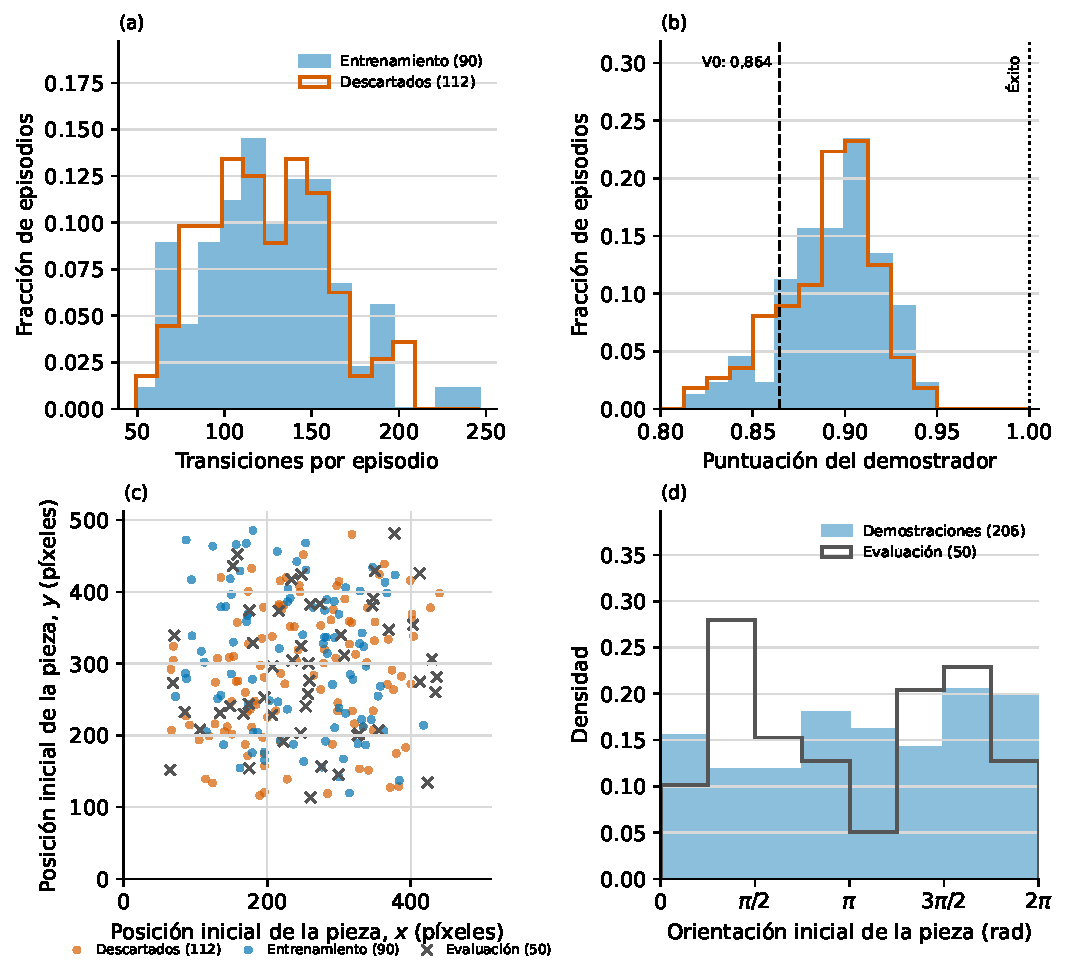
\includegraphics[width=\textwidth]{img/caracterizacion_dataset.pdf}
  \caption[Caracterizaci\'on del conjunto de demostraciones de
    Push-T.]{Caracterizaci\'on del conjunto de demostraciones de Push-T: (a) longitud de los
    episodios; (b) puntuaci\'on del demostrador, con el m\'aximo de V0 y el umbral de
    \'exito; (c) posici\'on inicial de la pieza, con las \num{50} condiciones de
    evaluaci\'on superpuestas; (d) orientaci\'on inicial de la pieza.}
  \label{fig:caracterizacion-dataset}
  \fuente{elaboraci\'on propia}
\end{figure}

El argumento que descarta un sesgo de selecci\'on es el procedimiento, no una prueba
estad\'istica: el reparto responde a un sorteo aleatorio uniforme sobre los \'indices de
episodio, sin ning\'un criterio de calidad, longitud ni dificultad. Un sorteo uniforme no
puede introducir sesgo sistem\'atico por construcci\'on.

Las comparaciones entre los dos subconjuntos cumplen aqu\'i un papel distinto y m\'as
modesto, el de comprobaci\'on descriptiva de que el sorteo se ejecut\'o como se describe.
Se presentan como tama\~nos de efecto con su incertidumbre, y no como valores $p$, porque
no rechazar la igualdad no demuestra equivalencia. Los episodios de entrenamiento son, en
media, \num{2.4} transiciones m\'as largos que los descartados, con un intervalo BCa al
\SI{95}{\percent} de {[\num{-7.7};\,\num{12.6}]} sobre una longitud media de \num{126}, es
decir menos del \SI{10}{\percent} de esa media en cualquiera de los dos extremos. En
puntuaci\'on del demostrador la diferencia es de \num{0.004}, con intervalo
{[\num{-0.004};\,\num{0.011}]}, un orden de magnitud por debajo de las diferencias entre
variantes que este trabajo interpreta. El $\delta$ de Cliff, que mide la probabilidad de
que un episodio de un subconjunto supere a uno del otro, vale \num{0.026} en longitud y
\num{0.085} en puntuaci\'on, ambos dentro de lo que se considera un efecto despreciable.
El mismo criterio se aplica a la comparaci\'on entre las condiciones iniciales de
entrenamiento y las \num{50} de evaluaci\'on, superpuestas en la
\cref{fig:caracterizacion-dataset}: los estad\'isticos de Kolmogorov-Smirnov sobre la
posici\'on del efector, la posici\'on de la pieza y su orientaci\'on quedan entre
\num{0.232} y \num{0.696} en valor $p$, sin que de ello se concluya equivalencia. En
cambio, el efecto de aprovechar tambi\'en los \num{112} episodios descartados no se ha
medido y queda recogido en el \cref{sec:trabajo-futuro}.

La procedencia p\'ublica del conjunto no sustituye a la comprobaci\'on del archivo
concreto que se ha utilizado. La \cref{tab:integridad} recoge los controles de integridad
aplicados sobre \'el, junto con la huella que lo identifica de forma un\'ivoca.

\begin{table}[htbp]
  \centering
  \caption{Controles de integridad del archivo de demostraciones.}
  \label{tab:integridad}
  \small
  \begin{tabular}{lll}
    \toprule
    Control & Regla & Resultado \\
    \midrule
    Valores ausentes  & Ning\'un \texttt{NaN} en los cinco arreglos & \num{0} \\
    Valores infinitos & Ning\'un \texttt{Inf} en los cinco arreglos & \num{0} \\
    Longitud coherente & Todos los arreglos con \num{25650} filas & Cumple \\
    \'Indices de episodio & Estrictamente crecientes, \num{206} finales & Cumple \\
    Longitud de episodio & Entre \num{49} y \num{246} transiciones & Cumple \\
    Rango de la acci\'on & Coordenadas en $[\num{12};\ \num{511}]$ p\'ixeles & Cumple \\
    Rango del estado & Coordenadas en $[\num{0.0002};\ \num{510.96}]$ & Cumple \\
    Rango de la imagen & Intensidades en $[\num{65};\ \num{255}]$, \texttt{float32}
      & Cumple \\
    Estados duplicados & Filas de \texttt{state} repetidas & \num{0} \\
    Tama\~no en disco & Suma de los bloques del directorio & \SI{31.0}{\mega\byte} \\
    \bottomrule
  \end{tabular}
  \notatabla{Los controles se ejecutan sobre el propio archivo \texttt{zarr}, abierto en
    modo lectura y recorrido por bloques para no cargar en memoria los \SI{2.84}{\giga\byte}
    del arreglo de im\'agenes. La huella SHA-256 del \'arbol de ficheros, calculada sobre
    su contenido en orden determinista, es
    \texttt{c235ab79\dots 275e36a4}; el valor completo figura en la
    \cref{tab:identificadores}.}
  \fuente{elaboraci\'on propia}
\end{table}

Conviene precisar, por \'ultimo, que la evaluaci\'on no consume datos de este fichero. El
rendimiento se mide ejecutando la pol\'itica en el simulador sobre condiciones iniciales
generadas de forma independiente, seg\'un se detalla en el \cref{sec:evaluacion}.

\section{Arquitectura de la pol\'itica}
\label{sec:arquitectura}

\textit{Diffusion Policy} modela la distribuci\'on condicional
$p(\mathbf{A}_t \mid \mathbf{O}_t)$, donde $\mathbf{O}_t$ agrupa las observaciones de los
\'ultimos $T_o$ instantes y $\mathbf{A}_t$ es una secuencia de $T_p$ acciones futuras
\cite{chi2025diffusion}. El muestreo de esa distribuci\'on se realiza mediante un modelo
probabil\'istico de difusi\'on con eliminaci\'on de ruido (\textit{Denoising Diffusion
Probabilistic Model}, DDPM) \cite{ho2020ddpm}.

El planificador de ruido fija una sucesi\'on $\beta_1,\dots,\beta_K$ y, a partir de ella,
$\alpha_k = 1-\beta_k$ y $\bar{\alpha}_k = \prod_{j=1}^{k}\alpha_j$. El proceso directo
perturba una secuencia de acciones real $\mathbf{A}^0_t$ interpolando entre la se\~nal
limpia y ruido gaussiano $\epsilon\sim\mathcal{N}(0,\mathbf{I})$, con los coeficientes que
recoge la \cref{eq:proceso-directo} del \cref{cap:estado-del-arte}:

\begin{equation}
  \mathbf{A}^{k}_t = \sqrt{\bar{\alpha}_k}\,\mathbf{A}^0_t
    + \sqrt{1-\bar{\alpha}_k}\;\epsilon .
  \label{eq:perturbacion}
\end{equation}

La red $\epsilon_\theta$ se ajusta para predecir ese ruido a partir del estado perturbado,
del \'indice de paso y de la observaci\'on. La funci\'on de p\'erdida es el error
cuadr\'atico medio sobre el ruido, recogido en la \cref{eq:perdida}.

\begin{equation}
  \mathcal{L} = \mathbb{E}_{k,\,\epsilon}\left[\left\lVert \epsilon -
    \epsilon_\theta\!\left(\mathbf{O}_t,\;
      \sqrt{\bar{\alpha}_k}\,\mathbf{A}^0_t + \sqrt{1-\bar{\alpha}_k}\,\epsilon,\; k\right)
    \right\rVert^2\right]
  \label{eq:perdida}
\end{equation}

En la \cref{eq:perdida}, el \'indice $k$ se muestrea de forma uniforme en
$\{1,\dots,K\}$ y determina, a trav\'es de $\bar{\alpha}_k$, la magnitud del ruido
inyectado. La observaci\'on $\mathbf{O}_t$ act\'ua como condicionamiento, no como variable
generada, lo que reduce el coste de inferencia. Por tanto, la calidad de la
representaci\'on visual condiciona directamente lo que la red generativa puede aprender.

Durante la inferencia, la pol\'itica parte de una secuencia de ruido puro
$\mathbf{A}^K_t\sim\mathcal{N}(0,\mathbf{I})$ y aplica $K$ transiciones inversas seg\'un la
\cref{eq:muestreo}.

\begin{equation}
  \mathbf{A}^{k-1}_t = \frac{1}{\sqrt{\alpha_k}}\left(\mathbf{A}^{k}_t -
    \frac{\beta_k}{\sqrt{1-\bar{\alpha}_k}}\;
    \epsilon_\theta\!\left(\mathbf{O}_t,\, \mathbf{A}^{k}_t,\, k\right)\right)
    + \sigma_k\,\mathbf{z},
  \qquad \mathbf{z}\sim\mathcal{N}(0,\mathbf{I})
  \label{eq:muestreo}
\end{equation}

La \cref{eq:muestreo} es la forma concreta que adoptan los coeficientes gen\'ericos
$\alpha$, $\gamma$ y $\sigma$ del muestreo DDPM: $\alpha = \alpha_k^{-1/2}$,
$\gamma = \beta_k(1-\bar{\alpha}_k)^{-1/2}$ y, con la varianza fija menor que emplea la
configuraci\'on de este trabajo,
$\sigma_k^2 = \tfrac{1-\bar{\alpha}_{k-1}}{1-\bar{\alpha}_k}\,\beta_k$. El t\'ermino
$\mathbf{z}$ se anula en el \'ultimo paso, $k=1$. El ruido fresco que se a\~nade en los
dem\'as preserva el car\'acter estoc\'astico del muestreo y, con ello, la capacidad de
representar varios modos de acci\'on.

El planificador concreto es el DDPM con $K = \num{100}$ pasos, id\'entico en entrenamiento
y en inferencia, sin acelerarlo mediante muestreadores impl\'icitos. Su sucesi\'on de
$\beta_k$ sigue el plan de coseno al cuadrado, definido por
$\bar{\alpha}_k = f(k)/f(0)$ con
$f(k) = \cos^2\!\left(\tfrac{k/K + s}{1+s}\cdot\tfrac{\pi}{2}\right)$ y
$s = 0{,}008$, y los $\beta_k$ resultantes se acotan superiormente en $0{,}999$ para
evitar la singularidad final. La red predice el ruido y no la muestra limpia, y la
estimaci\'on intermedia de $\mathbf{A}^0_t$ se recorta al intervalo $[-1,1]$ en el que se
normalizan las acciones. Con este plan, los par\'ametros de inicio y fin de una
progresi\'on lineal de $\beta$ no intervienen.

Las acciones generadas se aplican bajo un esquema de horizonte deslizante. La pol\'itica
recibe $T_o = 2$ observaciones, predice $T_p = 16$ acciones y ejecuta \'unicamente las
$T_a = 8$ primeras antes de replanificar \cite{chi2025diffusion}. Esta configuraci\'on
equilibra la consistencia temporal de la trayectoria con la capacidad de reaccionar ante
cambios en la escena.

La red $\epsilon_\theta$ es una red convolucional unidimensional con arquitectura en U y
dimensiones de canal \num{512}, \num{1024} y \num{2048} en sus tres niveles de
submuestreo. El vector de observaci\'on se inyecta como condicionamiento global en cada
capa mediante modulaci\'on lineal por caracter\'isticas (\textit{Feature-wise Linear
Modulation}, FiLM) \cite{perez2018film}. Este bloque concentra unos \num{277} millones de
par\'ametros y, por tanto, domina el coste de entrenamiento.

Delante de la red generativa opera el codificador de observaciones. Dicho m\'odulo aplica
las transformaciones de imagen propias de cada arquitectura, extrae un vector de
caracter\'isticas visuales y lo concatena con el estado del efector. La configuraci\'on de
referencia empleada aqu\'i utiliza una ResNet-18 \cite{he2016resnet} entrenada desde cero
cuya capa de clasificaci\'on se sustituye por la identidad, de modo que la agregaci\'on
espacial es el promediado global de la propia red. La \'unica modificaci\'on estructural
consiste en reemplazar la normalizaci\'on por lotes por normalizaci\'on por grupos
\cite{wu2018groupnorm}, ya que la primera interfiere con la media m\'ovil exponencial de
los pesos.

Conviene precisarlo porque el art\'iculo original describe adem\'as un \textit{spatial
softmax} que conserva la localizaci\'on de las activaciones \cite{levine2016visuomotor}.
Esa variante corresponde al codificador basado en \textit{robomimic} y no a la
configuraci\'on de Push-T con im\'agenes que este trabajo reproduce, donde el m\'odulo
codificador aplica \'unicamente redimensionado, recorte y normalizaci\'on antes de la red
convolucional. Ninguna de las cinco variantes de este estudio emplea, por tanto,
\textit{spatial softmax}: V0, V1 y V2 agregan por promediado global y V3 y V4 toman el
componente de clase del transformador.

\section{Variantes del codificador visual}
\label{sec:variantes}

Se definen cinco variantes, identificadas de V0 a V4, que modifican el bloque visual y el
tratamiento de sus pesos. La \cref{tab:variantes} resume su configuraci\'on. Las tres
primeras comparten arquitectura convolucional y permiten contrastar estrategias de
entrenamiento; las dos \'ultimas introducen transformadores de visi\'on preentrenados con
objetivos distintos.

\begin{table}[htbp]
  \centering
  \caption{Configuraci\'on de las cinco variantes del codificador visual evaluadas.}
  \label{tab:variantes}
  \small
  \begin{tabular}{lllcc c}
    \toprule
    Variante & Codificador visual & Pesos iniciales & Estrategia &
      \multicolumn{2}{c}{Par\'ametros (millones)} \\
    \cmidrule(lr){5-6}
     &  &  &  & Totales & Entrenables \\
    \midrule
    V0 & ResNet-18       & Aleatorios  & Desde cero  & \num{288} & \num{288} \\
    V1 & ResNet-18       & ImageNet-1k & Congelado   & \num{288} & \num{277} \\
    V2 & ResNet-18       & ImageNet-1k & Ajuste fino & \num{288} & \num{288} \\
    V3 & DINOv2 ViT-S/14 & LVD-142M    & Congelado   & \num{299} & \num{277} \\
    V4 & CLIP ViT-B/16   & WIT-400M    & Congelado   & \num{363} & \num{277} \\
    \bottomrule
  \end{tabular}
  \fuente{elaboraci\'on propia}
\end{table}

\divisionmenor{V0: l\'inea base entrenada desde cero}

La variante V0 reproduce la configuraci\'on original de \textit{Diffusion Policy}
\cite{chi2025diffusion}. Emplea una ResNet-18 con pesos aleatorios, opera sobre la imagen
a su resoluci\'on nativa de \num{96} p\'ixeles y aplica recorte aleatorio como \'unico
aumento de datos. El codificador se entrena de extremo a extremo junto con la red
generativa y constituye la referencia frente a la que se comparan las dem\'as variantes.

\divisionmenor{V1 y V2: transferencia desde ImageNet}

Las variantes V1 y V2 parten de una ResNet-18 preentrenada sobre ImageNet-1k
\cite{deng2009imagenet} y difieren en el tratamiento de sus pesos. En V1 el codificador
permanece congelado, de modo que act\'ua como extractor fijo de caracter\'isticas; en V2
sus pesos se actualizan junto con el resto de la pol\'itica. Ambas redimensionan la imagen
a \num{224} p\'ixeles por interpolaci\'on bilineal y aplican la normalizaci\'on est\'andar
de ImageNet, con id\'enticas constantes de media y desviaci\'on t\'ipica.

Sin embargo, \textbf{V1 y V2 no parten del mismo archivo de pesos}, y el contraste entre
ambas no puede leerse como el efecto aislado de la estrategia de entrenamiento. V1 carga
el modelo \texttt{resnet18} de \texttt{timm} con su etiqueta por defecto,
\texttt{resnet18.a1\_in1k}, obtenida con la receta A1 de \textit{ResNet strikes back}
\cite{wightman2021resnetsb}; V2 carga el modelo \texttt{resnet18} de
\texttt{torchvision} con la enumeraci\'on \texttt{ResNet18\_Weights.IMAGENET1K\_V1}, que
corresponde a la receta original de la biblioteca. Ambos son ResNet-18 ajustadas sobre
ImageNet-1k, pero proceden de procedimientos de entrenamiento distintos. La comprobaci\'on
es directa: como el codificador de V1 permanece congelado, los \num{120} tensores de su
punto de control deben coincidir con los pesos de partida. Comparados tensor a tensor,
coinciden de forma exacta con \texttt{resnet18.a1\_in1k} y no coincide ninguno con
\texttt{IMAGENET1K\_V1}. El \cref{sec:entorno} recoge el procedimiento, su resultado y los
identificadores completos de ambos archivos de pesos.

En consecuencia, la diferencia observada entre V1 y V2 combina la estrategia de
adaptaci\'on con el origen de los pesos, y este trabajo no la atribuye a la primera. Un
dise\~no que aislara la estrategia deber\'ia inicializar ambas desde el mismo archivo y
duplicar el estado antes de congelar una de las copias; queda descrito en el
\cref{sec:trabajo-futuro}.

El contraste entre V0 y las dos variantes preentrenadas tampoco aisla el efecto de la
inicializaci\'on, ya que el preprocesado y la configuraci\'on interna viajan con los
pesos. La \cref{tab:preprocesado} detalla la cadena completa de cada variante. Entre V0 y
V2 var\'ian de forma conjunta tres factores: los pesos iniciales, la resoluci\'on efectiva
de entrada junto con el recorte aleatorio y la capa de normalizaci\'on interna de la red,
que en V0 es por grupos y en V1 a V4 por lotes. Entre V0 y V1 se a\~nade un cuarto, el
entrenamiento conjunto del codificador frente a su congelaci\'on; y frente a V3 y V4
cambia adem\'as la arquitectura. Por tanto, esas comparaciones deben leerse sobre el
bloque visual completo y no sobre ninguno de sus factores por separado. Los entrenamientos
que los separar\'ian se describen en el \cref{sec:trabajo-futuro}.

\begin{table}[htbp]
  \centering
  \caption{Cadena de preprocesado de la imagen por variante, desde el fotograma
           renderizado hasta el tensor que recibe la red.}
  \label{tab:preprocesado}
  \small
  \begin{tabular}{llllll}
    \toprule
    Variante & Entrada & Redimensionado & Recorte & Normalizaci\'on & Tensor final \\
    \midrule
    V0 & \num{96}$\times$\num{96} & --- & \num{76}$\times$\num{76} aleatorio$^{*}$
       & ImageNet & \num{76}$\times$\num{76} \\
    V1 & \num{96}$\times$\num{96} & \num{224}$\times$\num{224} bilineal & ---
       & ImageNet & \num{224}$\times$\num{224} \\
    V2 & \num{96}$\times$\num{96} & \num{224}$\times$\num{224} bilineal & ---
       & ImageNet & \num{224}$\times$\num{224} \\
    V3 & \num{96}$\times$\num{96} & \num{224}$\times$\num{224} bilineal & ---
       & ImageNet & \num{224}$\times$\num{224} \\
    V4 & \num{96}$\times$\num{96} & \num{224}$\times$\num{224} bilineal & ---
       & CLIP & \num{224}$\times$\num{224} \\
    \bottomrule
  \end{tabular}
  \fuente{elaboraci\'on propia}
\end{table}

Tres precisiones sobre la \cref{tab:preprocesado}. Primera, el recorte de V0 es aleatorio
durante el entrenamiento y central en evaluaci\'on, de modo que el tensor mide siempre
\num{76}$\times$\num{76} y el aumento de datos solo act\'ua en el ajuste; es la \'unica
variante con aumento. Segunda, la normalizaci\'on ImageNet emplea las mismas constantes en
las cuatro variantes que la usan, media $(0{,}485;\ 0{,}456;\ 0{,}406)$ y desviaci\'on
t\'ipica $(0{,}229;\ 0{,}224;\ 0{,}225)$, aunque en V0 y V2 la aplica el m\'odulo
codificador y en V1 y V3 la aplica el propio envoltorio del modelo preentrenado. Tercera,
la normalizaci\'on de V4 emplea las constantes de CLIP, media $(0{,}481;\ 0{,}458;\
0{,}408)$ y desviaci\'on t\'ipica $(0{,}269;\ 0{,}261;\ 0{,}276)$, tal como exigen sus
pesos.

\divisionmenor{V3 y V4: transformadores de visi\'on preentrenados}

Las variantes V3 y V4 sustituyen la red convolucional por un transformador de visi\'on
\cite{dosovitskiy2021vit}. V3 utiliza DINOv2 ViT-S/14, preentrenado de forma
autosupervisada sobre el corpus LVD-142M \cite{oquab2024dinov2}. V4 utiliza CLIP ViT-B/16,
preentrenado con supervisi\'on de lenguaje natural sobre pares de imagen y texto
\cite{radford2021clip}. En ambos casos los pesos permanecen congelados, decisi\'on que
impone la memoria gr\'afica disponible. La medida recogida en la \cref{tab:memoria-gpu} la
respalda: el ajuste fino de la ResNet-18 de V2, con once millones de par\'ametros en el
codificador, ya reclama m\'as memoria de la que tiene la tarjeta y solo se completa porque
el controlador respalda el exceso con memoria del sistema, a costa de triplicar el tiempo
por \'epoca. Los dos transformadores aportan \num{22} y \num{86} millones de par\'ametros a
ese bloque, seg\'un se deduce de la \cref{tab:variantes}, de modo que ajustarlos agravar\'ia
el problema en lugar de aliviarlo.

Dado que la dimensi\'on de salida de estos modelos no coincide con la de la ResNet-18, se
a\~nade una capa lineal de proyecci\'on que reduce el descriptor a \num{512} componentes.
Dicha capa s\'i se entrena, puesto que forma parte de la pol\'itica y no del modelo
preentrenado. Los codificadores preentrenados se cargan mediante la biblioteca
\texttt{timm} \cite{wightman2019timm}, salvo la ResNet-18 de V2, que procede de
\texttt{torchvision}.

\section{Protocolo de entrenamiento}
\label{sec:protocolo}

Las variantes comparten los hiperpar\'ametros recogidos en la
\cref{tab:hiperparametros}, salvo las dos excepciones indicadas en ella. El presupuesto se
redujo durante la campa\~na conforme aumentaba el coste observado: \num{500} \'epocas para
V0 y V1, \num{300} para V2 y V3, y \num{200} para V4. Estos valores quedan muy por debajo
de las \num{3000} \'epocas del art\'iculo original. Dentro de cada presupuesto se aplica el
criterio de parada que se precisa m\'as adelante.

\begin{table}[htbp]
  \centering
  \caption{Hiperpar\'ametros de entrenamiento de las cinco variantes.}
  \label{tab:hiperparametros}
  \small
  \begin{tabular}{ll}
    \toprule
    Par\'ametro & Valor \\
    \midrule
    Horizonte de predicci\'on $T_p$        & \num{16} pasos \\
    Pasos de observaci\'on $T_o$           & \num{2} \\
    Pasos de acci\'on ejecutados $T_a$     & \num{8} \\
    Pasos de difusi\'on (entrenamiento e inferencia) & \num{100} \\
    Planificador de ruido                  & DDPM, varianza fija, predicci\'on de ruido \\
    Optimizador                            & AdamW \cite{loshchilov2019adamw} \\
    Tasa de aprendizaje                    & \num{1e-4}, decaimiento coseno \\
    Pasos de calentamiento                 & \num{500} \\
    Media m\'ovil exponencial de los pesos & Activada \\
    Tama\~no de lote                       & \num{64} (\num{32} en V3 y V4) \\
    Acumulaci\'on de gradiente             & \num{1} (\num{2} en V3 y V4) \\
    Tama\~no de lote efectivo              & \num{64} en las cinco variantes \\
    Presupuesto m\'aximo de \'epocas       & \num{500} (V0--V1); \num{300} (V2--V3);
                                               \num{200} (V4) \\
    Semilla                                & \num{42} \\
    \bottomrule
  \end{tabular}
  \fuente{elaboraci\'on propia}
\end{table}

Adem\'as del presupuesto, el tama\~no de lote de V3 y V4 se redujo a la mitad, ya que los
dos transformadores operan a \num{224} p\'ixeles y comprometen la memoria gr\'afica
disponible con lotes de \num{64} muestras. La reducci\'on se compensa acumulando el
gradiente durante dos lotes antes de cada actualizaci\'on, de modo que el tama\~no de lote
efectivo y el n\'umero de actualizaciones por \'epoca coinciden con los de V0, V1 y V2:
\num{336} lotes y \num{168} actualizaciones frente a \num{168} lotes y otras tantas
actualizaciones. Lo que s\'i cambia es el n\'umero de pasadas por el codificador, que se
duplica, y con \'el el tiempo por \'epoca. La \cref{tab:memoria-gpu} matiza esta
decisi\'on: con lote reducido V4 llega al \SI{90.3}{\percent} de la memoria de la tarjeta,
de modo que la reducci\'on estaba justificada, mientras que V3 se queda en el
\SI{78.2}{\percent} y dispon\'ia de m\'as margen. En V3 la medida no sostiene la necesidad
y la reducci\'on debe leerse como cautela y como forma de igualar las condiciones de los
dos transformadores.

Cada entrenamiento se lanza mediante un script de control que fija los par\'ametros de
ejecuci\'on, verifica la memoria disponible e impide que se ejecuten dos procesos de forma
simult\'anea. Esta salvaguarda responde a un incidente previo, en el que dos procesos
concurrentes sobre el mismo directorio de salida agotaron la memoria del sistema y
corrompieron el registro de m\'etricas.

La \cref{tab:config-efectiva} recoge la configuraci\'on que Hydra resolvi\'o
efectivamente para cada ejecuci\'on, tomada de los ficheros que el propio marco de
configuraci\'on escribe junto a los resultados. Se listan solo los par\'ametros que
difieren entre variantes; los comunes se enuncian bajo la tabla.

\begin{table}[htbp]
  \centering
  \caption{Configuraci\'on efectiva de las cinco ejecuciones. Solo se muestran los
    par\'ametros que difieren entre ellas.}
  \label{tab:config-efectiva}
  \small
  \begin{tabular}{lccccc}
    \toprule
    Par\'ametro & V0 & V1 & V2 & V3 & V4 \\
    \midrule
    Presupuesto de \'epocas   & \num{500} & \num{500} & \num{300} & \num{300} & \num{200} \\
    \'Epocas completadas      & \num{500} & \num{500} & \num{266} & \num{155} & \num{200} \\
    Tama\~no de lote          & \num{64} & \num{64} & \num{64} & \num{32} & \num{32} \\
    Acumulaci\'on de gradiente & \num{1} & \num{1} & \num{1} & \num{2} & \num{2} \\
    Lote efectivo             & \num{64} & \num{64} & \num{64} & \num{64} & \num{64} \\
    Actualizaciones por \'epoca & \num{168} & \num{168} & \num{168} & \num{168} & \num{168} \\
    Codificador congelado     & No & S\'i & No & S\'i & S\'i \\
    Normalizaci\'on de la red & Grupos & Lotes & Lotes & Capas & Capas \\
    Guardado cada (\'epocas)  & \num{50} & \num{50} & \num{50} & \num{10} & \num{10} \\
    \bottomrule
  \end{tabular}
  \notatabla{Par\'ametros comunes a las cinco ejecuciones: semilla \num{42}; optimizador
    AdamW \cite{loshchilov2019adamw} con tasa de aprendizaje \num{1e-4}, momentos
    $(0{,}95;\ 0{,}999)$, $\varepsilon = \num{1e-8}$ y decaimiento de pesos \num{1e-6};
    planificador de tasa de coseno con \num{500} pasos de calentamiento; media m\'ovil
    exponencial con potencia $0{,}75$ y valor m\'aximo $0{,}9999$; validaci\'on cada
    \'epoca; evaluaci\'on en el simulador cada \num{50} \'epocas con \num{8} procesos; y
    conservaci\'on de los tres mejores puntos de control seg\'un la puntuaci\'on de
    selecci\'on, adem\'as del \'ultimo. Las configuraciones completas y los registros de
    cada ejecuci\'on residen en el repositorio del trabajo \cite{britez2026repo}.}
  \fuente{elaboraci\'on propia}
\end{table}

Durante el entrenamiento se guarda un punto de control cada \num{50} \'epocas y se
conservan los tres mejores seg\'un la puntuaci\'on de evaluaci\'on. El modelo evaluado en
el \cref{cap:resultados} es el de mayor puntuaci\'on, criterio coherente con el empleado
en la literatura de la tarea \cite{mandlekar2021robomimic}.

El criterio de parada anticipada se apoya en esos mismos puntos de control. Un
entrenamiento se interrumpe cuando la puntuaci\'on de evaluaci\'on no supera su m\'aximo en
dos evaluaciones consecutivas, esto es, tras \num{100} \'epocas sin mejora, mientras la
p\'erdida de entrenamiento sigue descendiendo. Esa combinaci\'on apunta a sobreajuste, de
modo que prolongar la ejecuci\'on no aportar\'ia un punto de control mejor. La parada no se
aplica antes de la \'epoca \num{200}, para no interrumpir una variante de convergencia
lenta. El criterio no altera el modelo seleccionado, puesto que este se elige entre los
puntos de control ya guardados.

Este criterio no precedi\'o al experimento, sino que se adopt\'o durante su ejecuci\'on. Las
dos primeras variantes, V0 y V1, agotaron \num{500} \'epocas porque entonces no exist\'ia
regla de parada. La formulaci\'on anterior se fij\'o al observar sus curvas y se aplic\'o a
V2, detenida tras \num{266} \'epocas completas. V3 se interrumpi\'o manualmente tras
\num{155} \'epocas completas, es decir en la de \'indice \num{154}, antes del m\'inimo de
\num{200} que la propia regla fijaba, mientras que V4 agot\'o sus \num{200} \'epocas. Los
\'indices de \'epoca empiezan en cero, de modo que ambas cifras designan el mismo
instante; en el resto de la memoria se emplea siempre el recuento de \'epocas completas. Las decisiones se tomaron por inspecci\'on, no de forma autom\'atica.

Esta asimetr\'ia afecta al coste y a la selecci\'on del modelo. V3 y V4 solo disponen de
cuatro evaluaciones, frente a las diez de V0 y V1, por lo que tuvieron menos oportunidades
de alcanzar un m\'aximo tard\'io. El \cref{sec:coste} reconstruye el contrafactual bajo el
criterio aplicado de forma uniforme, dentro del presupuesto asignado a cada variante.

\section{Protocolo de evaluaci\'on}
\label{sec:evaluacion}

La evaluaci\'on se ejecuta cada \num{50} \'epocas sobre \num{56} condiciones iniciales del
simulador. Seis de ellas proceden de la distribuci\'on de entrenamiento y las \num{50}
restantes se generan con semillas de entorno reservadas, no empleadas durante el ajuste.
Las primeras permiten estimar el ajuste a los datos vistos; las segundas constituyen la
medida de rendimiento que se reporta.

Cada condici\'on inicial se resuelve en un episodio completo de bucle cerrado. La
pol\'itica recibe las observaciones, genera una secuencia de acciones, ejecuta las
primeras $T_a$ y repite el ciclo hasta alcanzar el l\'imite de pasos del episodio o
completar la tarea. Los pesos utilizados son los de la media m\'ovil exponencial, no los
del modelo instant\'aneo, tal como prescribe la implementaci\'on de referencia.

Las condiciones se agrupan en tandas de ocho procesos para no agotar la memoria del
sistema. Esta agrupaci\'on modifica el tiempo de ejecuci\'on de la evaluaci\'on, pero no las
m\'etricas resultantes, puesto que la agregaci\'on recorre las \num{56} condiciones con
independencia del n\'umero de procesos simult\'aneos.

\section{M\'etricas}
\label{sec:metricas}

La m\'etrica principal es la puntuaci\'on de cobertura de la tarea Push-T
\cite{chi2025diffusion}. Para un episodio $j$, se calcula en cada instante $t$ la
cobertura $c_{j,t}$, definida como la fracci\'on del \'area objetivo cubierta por la
pieza. La puntuaci\'on del episodio se obtiene seg\'un la \cref{eq:score}.

\begin{equation}
  s_j = \max_{1 \le t \le T} \min\!\left(\frac{c_{j,t}}{\tau},\, 1\right)
  \label{eq:score}
\end{equation}

En la \cref{eq:score}, $T$ es la duraci\'on m\'axima del episodio y $\tau$ el umbral de
cobertura que define el \'exito, fijado en \num{0.95} por la implementaci\'on de
referencia. La puntuaci\'on resulta as\'i continua y acotada en el intervalo unidad: vale
uno cuando la pieza alcanza el umbral en alg\'un instante y crece de forma proporcional a
la cobertura en caso contrario. Se toma el m\'aximo a lo largo del episodio, y no el valor
final, porque la pieza puede desplazarse tras alcanzar la posici\'on objetivo.

La m\'etrica que se reporta es la media de $s_j$ sobre los \num{50} episodios evaluados,
denominada puntuaci\'on media de evaluaci\'on. Junto a ella se reportan la desviaci\'on
t\'ipica y el error est\'andar de esos \num{50} valores, magnitudes que describen la
dispersi\'on de la propia m\'etrica. Se registran adem\'as cuatro cantidades auxiliares:
la p\'erdida de entrenamiento, la p\'erdida de validaci\'on, el error cuadr\'atico medio
de la acci\'on predicha y la puntuaci\'on media sobre las seis condiciones que la
implementaci\'on de referencia denomina de entrenamiento. Las dos primeras describen el
ajuste y su comparaci\'on es la que revela el sobreajuste.

Esa cuarta cantidad exige una advertencia. Sus seis condiciones iniciales son las de las
demostraciones \num{0} a \num{5}, y el sorteo descrito en el \cref{sec:datos} dej\'o las
seis fuera del subconjunto de entrenamiento. La puntuaci\'on que se obtiene sobre ellas no
mide, por tanto, el rendimiento en condiciones vistas durante el ajuste, y no se emplea en
esta memoria como indicio de sobreajuste.

El nombre de la m\'etrica principal requiere una precisi\'on. Las \num{50} condiciones se
generan con semillas reservadas y no intervienen en el ajuste de los pesos, pero se
eval\'uan cada \num{50} \'epocas y determinan qu\'e punto de control se conserva. Cumplen,
por tanto, la funci\'on de un conjunto de selecci\'on y no la de una evaluaci\'on final
independiente. El t\'ermino \textit{prueba} se reserva para la medida sobre el bloque
disjunto que describe el \cref{sec:seleccion-prueba}, donde se detallan tambi\'en el
estimando, las unidades experimentales y el tratamiento estad\'istico de las diferencias.

El coste computacional se caracteriza mediante cuatro indicadores. El primero es el
n\'umero de par\'ametros totales y entrenables de cada variante, recogido en la
\cref{tab:variantes}. El segundo es el tiempo por paso de optimizaci\'on, medido tras la
fase de calentamiento y agregado por \'epoca en la \cref{tab:coste}. El tercero es la
latencia de inferencia para un lote de tama\~no fijo. El cuarto es el pico de memoria
gr\'afica reservada durante el entrenamiento. Los dos \'ultimos se reportan en el
\cref{sec:coste-resultados}.

La latencia se desglosa en tres magnitudes, porque una sola oculta el efecto que se
estudia. Cada llamada a la pol\'itica ejecuta el codificador visual una vez y la red
generativa cien veces, de modo que el tiempo total lo domina un componente id\'entico en
las cinco variantes. Se reportan, por tanto, la latencia de la llamada completa, la del
codificador aislado y la de la llamada dividida entre las ocho acciones que emite, esta
\'ultima porque acota la frecuencia de control alcanzable. Las medidas se toman en
precisi\'on \texttt{float32}, con lotes de \num{1} y \num{8} muestras, y se resumen
mediante la mediana y el recorrido intercuart\'ilico de \num{50} repeticiones
cronometradas, precedidas de \num{20} descartadas. Las repeticiones se alternan entre
variantes por rondas, para que la deriva t\'ermica del equipo port\'atil afecte por igual
a todas.

El pico de memoria exige reproducir el paso de optimizaci\'on completo, ya que los
gradientes, los momentos de AdamW y la copia de la media m\'ovil son justamente lo que
ocupa la tarjeta. Se ejecutan doce pasos sobre lotes reales, con el tama\~no propio de cada
variante, y se registra la memoria reservada por el asignador. Se acompa\~na del pico en
inferencia, que describe lo que exigir\'ia un despliegue.

Ambas medidas se toman en entornos de ejecuci\'on distintos y esa diferencia se declara en
cada tabla. La latencia se mide en el entorno de inferencia sobre Windows y el pico de
memoria en el entorno de WSL en el que se entren\'o, puesto que el asignador de memoria de
PyTorch cambi\'o entre ambas versiones y una cifra tomada en Windows no describir\'ia las
ejecuciones recogidas en la \cref{tab:coste}. Dentro de cada indicador, las cinco variantes
comparten entorno.

\section{Selecci\'on del punto de control y prueba final}
\label{sec:seleccion-prueba}

Los conjuntos de condiciones iniciales cumplen dos funciones distintas que conviene no
confundir. El primero elige qu\'e punto de control representa a cada variante; el segundo
mide su rendimiento sin haber intervenido en esa elecci\'on. La
\cref{fig:flujo-evaluacion} resume el recorrido completo, desde los episodios de
demostraci\'on hasta la tabla de resultados finales.

\begin{figure}[htbp]
  \centering
  \begin{tikzpicture}[
      font=\footnotesize,
      caja/.style={draw, rounded corners=2pt, align=center, inner sep=4pt,
                   minimum height=13mm, text width=26mm},
      datos/.style={caja, fill=black!4},
      final/.style={caja, line width=0.9pt, fill=black!8},
      ancho/.style={final, text width=30mm},
      flecha/.style={-{Latex[length=2mm]}, thick},
      aporte/.style={flecha, densely dashed},
    ]
    \node[datos] (train) {\num{90} episodios\\ajuste de pesos};
    \node[datos, right=9mm of train] (ckpt) {\num{3} puntos de control\\guardados};
    \node[datos, right=9mm of ckpt] (elegido) {Punto de control\\congelado};
    \node[ancho, right=9mm of elegido] (tabla) {Resultados finales\\IC, Wilcoxon y Holm};

    \node[datos, below=7mm of train] (val)
      {\num{4} episodios\\p\'erdida de validaci\'on};
    \node[datos, below=7mm of elegido] (seleccion)
      {Selecci\'on\\\num{50} semillas\\\num{100000}--\num{100049}};
    \node[final, below=7mm of tabla] (prueba)
      {\textbf{Prueba}\\\num{200} semillas\\\num{200000}--\num{200199}};

    \draw[flecha] (train) -- (ckpt);
    \draw[flecha] (ckpt) -- (elegido);
    \draw[flecha] (elegido) -- (tabla);
    \draw[flecha] (seleccion) -- (elegido);
    \draw[flecha] (prueba) -- (tabla);
    \draw[aporte] (val) -- node[right=1pt, pos=0.45] {diagn\'ostico} (train);
  \end{tikzpicture}
  \caption[Flujo de ajuste, validaci\'on, selecci\'on y prueba.]{Flujo de ajuste,
    validaci\'on, selecci\'on y prueba. Las \num{50} semillas de selecci\'on solo alcanzan
    la tabla final a trav\'es del punto de control que congelan. Los \num{112} episodios
    restantes del conjunto de datos no intervienen en ninguna etapa.}
  \label{fig:flujo-evaluacion}
  \fuente{elaboraci\'on propia}
\end{figure}

\divisionmenor{Estimando y unidades experimentales}

El estimando primario es la puntuaci\'on media de cobertura de un punto de control fijo
sobre el generador de condiciones iniciales de Push-T. Se estima con las \num{200}
condiciones del bloque de prueba, muestreadas de ese generador mediante semillas
consecutivas. La variable de resultado secundaria es la tasa de \'exito, es decir, la
fracci\'on de condiciones cuya puntuaci\'on alcanza el umbral.

El estudio maneja tres unidades distintas y solo replica una de ellas. El episodio de
demostraci\'on construye las ventanas de entrenamiento; la condici\'on inicial eval\'ua un
punto de control ya fijado; la ejecuci\'on completa de entrenamiento permitir\'ia comparar
estrategias. Existen \num{90}, \num{200} y \num{1} unidades por variante en esos tres
niveles. Por tanto, la unidad de replicaci\'on de este trabajo es la condici\'on inicial:
las cifras estiman el rendimiento de cinco artefactos concretos, no el rendimiento
esperado de volver a entrenar cada estrategia. Esa restricci\'on se mantiene en las
conclusiones y se recoge en el \cref{sec:limitaciones}.

\divisionmenor{Bloque de prueba disjunto}

La prueba final emplea las semillas de entorno \num{200000} a \num{200199}. El bloque es
disjunto de las semillas \num{0} a \num{205} que generaron las demostraciones y de las
\num{50} de selecci\'on, condici\'on que el programa de evaluaci\'on comprueba antes de
ejecutar nada. El desplazamiento a \num{200000}, en lugar de continuar la serie de
selecci\'on, evita cualquier ambig\"uedad al leer las tablas.

Se eval\'ua una sola vez cada uno de los cinco puntos de control ya seleccionados, con los
pesos de la media m\'ovil exponencial y la misma configuraci\'on del simulador que durante
el entrenamiento. Ninguna decisi\'on posterior a esa medida modifica qu\'e punto de control
representa a cada variante. El protocolo, incluidas las semillas, el tama\~no de muestra,
las variables de resultado y el an\'alisis, se fij\'o por escrito y se registr\'o en el
repositorio antes de ejecutar la evaluaci\'on.

Conviene declarar el l\'imite de este procedimiento. Durante el entrenamiento solo se
conservaron los tres mejores puntos de control de cada variante seg\'un la puntuaci\'on de
selecci\'on, de modo que el conjunto de candidatos ya viene filtrado por esa m\'etrica. El
bloque disjunto acota el sesgo de selecci\'on, pero no lo elimina por completo.

\divisionmenor{Ruido de difusi\'on sincronizado}

La pol\'itica parte de ruido y a\~nade ruido en cada uno de los \num{100} pasos de
difusi\'on, seg\'un la \cref{eq:muestreo}. Dos variantes evaluadas en la misma condici\'on
inicial no formar\'ian un par comparable si cada una recibiera una realizaci\'on distinta
de ese ruido. Para evitarlo se aplica la t\'ecnica de los n\'umeros aleatorios comunes: el
generador se siembra antes de cada llamada a la pol\'itica en funci\'on de la posici\'on
del ciclo de control, con una semilla base com\'un a las cinco variantes.

El esquema produce ruido id\'entico entre variantes porque todas comparten la forma del
tensor de ruido, el n\'umero de tandas y el n\'umero de llamadas por tanda. En modo
evaluaci\'on, adem\'as, el recorte aleatorio de V0 pasa a ser un recorte central, de modo
que el codificador no consume n\'umeros aleatorios. Cada condici\'on se resuelve con una
sola trayectoria de difusi\'on, compartida por las cinco variantes, y el estimando queda
definido en consecuencia.

\divisionmenor{Especificaci\'on estad\'istica}

Las diferencias se calculan por pares, emparejando cada variante con las dem\'as sobre la
misma condici\'on inicial. Cada diferencia media se acompa\~na de un intervalo de confianza
del \SI{95}{\percent} obtenido por \textit{bootstrap} BCa con \num{10000} remuestreos de
los pares y semilla fija. Este m\'etodo se elige porque no supone normalidad de las
diferencias y corrige el sesgo y la asimetr\'ia de la distribuci\'on remuestreada.

El contraste preregistrado es la prueba de los rangos con signo de Wilcoxon. Los pares
nulos se descartan seg\'un el criterio del propio Wilcoxon. Con \num{200} pares la
distribuci\'on exacta no resulta aplicable, de modo que se usa la aproximaci\'on normal con
correcci\'on de continuidad; el m\'etodo empleado se registra en cada fila de la tabla de
contrastes.

A ese contraste se a\~nade una prueba de permutaci\'on sobre la diferencia media, por
inversi\'on de signo de los pares, con \num{10000} permutaciones y semilla fija. Su
inclusi\'on responde a una objeci\'on pertinente: el estimando primario declarado es una
diferencia de medias, y Wilcoxon opera sobre los rangos de las diferencias, no sobre su
media. La prueba de permutaci\'on toma como estad\'istico la propia media y contrasta la
simetr\'ia de las diferencias en torno a cero, de modo que apunta a la cantidad que la
memoria reporta. Se declara sin ambig\"uedad como \textbf{an\'alisis post hoc}: no figuraba
en el protocolo preregistrado y se a\~nadi\'o despu\'es de observar el bloque de prueba.
Ambos contrastes se reportan juntos en el \cref{sec:prueba-final} y ninguno sustituye al
otro; donde discrepan, la memoria adopta la lectura m\'as conservadora.

La familia de hip\'otesis la forman las diez comparaciones por pares de la variable de
resultado principal, y cada contraste se corrige sobre su propia familia de diez. La tasa
de \'exito es una variable secundaria y descriptiva: se acompa\~na de intervalos de Wilson
y no entra en ninguna familia corregida ni sostiene conclusi\'on alguna por s\'i sola. Sus valores $p$ se ajustan mediante el procedimiento secuencial de Holm, que controla el
error familiar sin suponer independencia entre contrastes, y la significaci\'on se
determina sobre los valores ajustados con un umbral de \num{0.05}. Los intervalos de
confianza no incorporan ese ajuste y se presentan como descriptivos.

Estas medidas caracterizan la variabilidad debida a las condiciones iniciales y, gracias a
la sincronizaci\'on del ruido, no la mezclan con la del muestreo de difusi\'on. No
sustituyen, en cambio, a la variabilidad entre semillas de entrenamiento, que exigir\'ia
repetir los ajustes y queda fuera del alcance fijado en el \cref{sec:alcance}.

\section{Comparaci\'on con la implementaci\'on de referencia}
\label{sec:comparacion-paper}

El \cref{sec:seleccion-prueba} ordena cinco artefactos propios entre s\'i. Queda abierta una
pregunta distinta y previa: si V0, que reproduce la configuraci\'on visual de la
implementaci\'on de referencia, alcanza el rendimiento del punto de control que sus autores
publicaron para Push-T \cite{chi2023diffusion}. El presente apartado fija el protocolo de
ese contraste, registrado en el repositorio antes de ejecutar la medida.

\divisionmenor{Artefacto de referencia y factores confundidos}

El punto de control publicado, designado en adelante V\textsubscript{pub}, no constituye una
sexta variante del experimento. Su codificador procede de la biblioteca robomimic
\cite{mandlekar2021robomimic} y agrega la salida convolucional mediante un
\textit{spatial softmax} de \num{32} puntos clave seguido de una capa lineal, mientras que
las cinco variantes de este trabajo emplean promediado global o componente de clase. La
\cref{tab:comparacion-factores} detalla qu\'e comparten los dos artefactos y en qu\'e
difieren.

\begin{table}[htbp]
  \centering
  \caption{Elementos comunes y factores que difieren entre V0 y el punto de control
    publicado.}
  \label{tab:comparacion-factores}
  \small
  \scriptsize
  \begin{tabular}{p{30mm} p{40mm} p{40mm}}
    \toprule
    Elemento & V0 & V\textsubscript{pub} \\
    \midrule
    \multicolumn{3}{l}{\textit{Comunes}} \\
    Datos y partici\'on & \multicolumn{2}{p{82mm}}{\num{90} episodios de ajuste y \num{4} de
      validaci\'on, con la misma semilla de partici\'on} \\
    Red generativa & \multicolumn{2}{p{82mm}}{U-Net condicional, canales \num{512},
      \num{1024} y \num{2048}} \\
    Muestreo & \multicolumn{2}{p{82mm}}{DDPM con \num{100} pasos} \\
    Horizontes & \multicolumn{2}{p{82mm}}{predicci\'on \num{16}, observaci\'on \num{2},
      ejecuci\'on \num{8}} \\
    \midrule
    \multicolumn{3}{l}{\textit{Difieren}} \\
    Agregaci\'on espacial & Promediado global & \textit{Spatial softmax} de \num{32} puntos
      clave \\
    Recorte & \num{76}$\times$\num{76} & \num{84}$\times$\num{84} \\
    Presupuesto y punto de control & \num{500} \'epocas, \'epoca \num{350} & calendario de
      \num{3050} \'epocas, \'epoca \num{500} \\
    Bloque de selecci\'on & \numrange{100000}{100049} & \numrange{4300000}{4300049} \\
    Implementaci\'on & Bifurcaci\'on propia & C\'odigo original de los autores \\
    \bottomrule
  \end{tabular}
  \notatabla{Los cuatro factores de la mitad inferior var\'ian de forma conjunta, de modo que
    el contraste no aisla ninguno de ellos por separado.}
  \fuente{elaboraci\'on propia}
\end{table}

Cuatro factores var\'ian a la vez. El alcance del contraste es, en consecuencia, el de una
comparaci\'on entre dos artefactos completos: determina si el modelo obtenido en este
trabajo iguala al publicado, no a qu\'e componente se debe la diferencia. La unidad sobre la
que se infiere sigue siendo el artefacto entrenado.

\divisionmenor{Dise\~no pareado y realizaciones del ruido}

Ambos artefactos se eval\'uan sobre las mismas \num{200} condiciones iniciales del bloque
\numrange{200000}{200199}, de manera que la comparaci\'on queda pareada por condici\'on. Ese
bloque es adem\'as disjunto de las \num{50} semillas con las que los autores seleccionaron su
punto de control, extremo que el programa de evaluaci\'on comprueba antes de ejecutar nada.

A diferencia del \cref{sec:seleccion-prueba}, cada artefacto se eval\'ua con \textbf{dos
realizaciones del ruido de difusi\'on}, generadas a partir de dos semillas base declaradas de
antemano. Dentro de cada realizaci\'on se mantienen los n\'umeros aleatorios comunes entre
los dos artefactos. La ampliaci\'on responde a la limitaci\'on recogida en el
\cref{sec:limitaciones}: con una sola trayectoria, el estimando queda condicionado a esa
realizaci\'on concreta del ruido.

El estimando primario es, por tanto, la diferencia entre las puntuaciones medias de cobertura
de los dos artefactos sobre el generador de condiciones iniciales \textbf{y} sobre la
realizaci\'on del ruido. La unidad de observaci\'on sigue siendo la condici\'on inicial: las
dos realizaciones se promedian dentro de cada condici\'on antes de contrastar, de modo que el
an\'alisis opera sobre \num{200} diferencias independientes y no sobre \num{400}
observaciones anidadas. La varianza intracondici\'on entre realizaciones se reporta por
separado, como variable de resultado secundaria.

\divisionmenor{Contraste primario y margen de equivalencia}

El contraste primario es la prueba de permutaci\'on por inversi\'on de signo sobre la
diferencia media, bilateral, con \num{10000} permutaciones y semilla fija. Se adopta como
primaria, y no como complemento, porque su estad\'istico es la media, que es la cantidad
declarada en el estimando. La prueba de Wilcoxon se conserva como comprobaci\'on de robustez.
Al existir un \'unico contraste primario entre dos artefactos, no hay familia de
hip\'otesis que corregir, y la familia de diez comparaciones del \cref{sec:prueba-final}
permanece intacta.

El dise\~no incorpora adem\'as un an\'alisis de equivalencia, ausente en el protocolo
anterior. Se fija un margen pr\'actico $\delta = \num{0.05}$ antes de observar los datos. Su
justificaci\'on es emp\'irica: evaluaciones repetidas de estados de entrenamiento casi
id\'enticos se separan entre \num{0.047} y \num{0.097} puntos, del orden de un error
est\'andar de la propia medida, de modo que una diferencia inferior a \num{0.05} no supera la
dispersi\'on de repetir la medici\'on. Ese margen equivale, asimismo, a menos de la cuarta
parte de la menor diferencia que el \cref{sec:prueba-final} da por establecida. Se declara
equivalencia pr\'actica cuando el intervalo BCa al \SI{90}{\percent} de la diferencia media
queda contenido en $(-\delta, +\delta)$. Ese criterio equivale al procedimiento de las dos
pruebas unilaterales (TOST, \textit{two one-sided tests}) con $\alpha = \num{0.05}$.

La combinaci\'on de ambas decisiones produce los cuatro desenlaces de la
\cref{tab:regla-decision}, fijados antes de observar los datos.

\begin{table}[htbp]
  \centering
  \caption{Regla de decisi\'on del contraste, fijada antes de observar los datos.}
  \label{tab:regla-decision}
  \small
  \scriptsize
  \begin{tabular}{p{32mm} p{40mm} p{40mm}}
    \toprule
    & $p < \num{0.05}$ & $p \geq \num{0.05}$ \\
    \midrule
    IC \SI{90}{\percent} dentro de $\pm\delta$ & Diferencia detectable, pr\'acticamente
      irrelevante & Equivalencia pr\'actica \\
    IC \SI{90}{\percent} fuera de $\pm\delta$ & Diferencia relevante & Indeterminado, por
      potencia insuficiente \\
    \bottomrule
  \end{tabular}
  \notatabla{El valor $p$ procede de la prueba de permutaci\'on y el intervalo del
    \textit{bootstrap} BCa de \num{10000} remuestreos. La casilla inferior derecha no
    autoriza a concluir equivalencia, puesto que la ausencia de significaci\'on y la
    imprecisi\'on del intervalo son compatibles con diferencias mayores que el margen.}
  \fuente{elaboraci\'on propia}
\end{table}

La variable de resultado secundaria es la tasa de \'exito, contrastada por realizaci\'on
mediante la prueba exacta de McNemar sobre los pares discordantes. No se agrega entre
realizaciones, puesto que el promedio de dos indicadores binarios no constituye un indicador.

\divisionmenor{Comprobaciones previas y alcance del preregistro}

Tres comprobaciones con criterio num\'erico fijado de antemano preceden a la medida. La
primera reeval\'ua V0 sobre las ocho primeras condiciones del bloque con la semilla base
original y exige coincidencia exacta con el resultado ya registrado; de ella depende que ese
resultado pueda reutilizarse como primera realizaci\'on en lugar de repetirlo. La segunda
eval\'ua V\textsubscript{pub} sobre el bloque de \num{50} semillas con el que sus autores lo
reportan y exige que la media se aleje menos de \num{0.07}, dos errores est\'andar, de la
cifra publicada; sin ella, la ruta de inferencia empleada aqu\'i no reproducir\'ia la de los
autores y el contraste carecer\'ia de sentido. La tercera compara el primer tensor de ruido
que muestrean ambos artefactos con la misma semilla y verifica que los n\'umeros aleatorios
comunes quedan alineados.

Conviene precisar, por \'ultimo, el alcance del preregistro. Las puntuaciones de V0 en la
primera realizaci\'on ya exist\'ian, puesto que proceden del \cref{sec:prueba-final}. El
documento fija por adelantado el artefacto de referencia completo, la segunda realizaci\'on
de ambos artefactos y la totalidad del an\'alisis, pero no puede fijar lo ya observado. Esa
asimetr\'ia se declara y no se subsana.

\section{Entorno de ejecuci\'on y reproducibilidad}
\label{sec:entorno}

Todos los experimentos se ejecutan sobre un \'unico equipo port\'atil, cuyas
caracter\'isticas se recogen en la \cref{tab:entorno}. El c\'omputo no se reparte entre
varias m\'aquinas ni se recurre a servicios en la nube, de modo que las medidas de coste
del \cref{sec:coste} son directamente comparables entre variantes.

\begin{table}[htbp]
  \centering
  \caption{Plataforma de ejecuci\'on de los experimentos.}
  \label{tab:entorno}
  \small
  \begin{tabular}{lll}
    \toprule
    Bloque & Componente & Caracter\'isticas \\
    \midrule
    \multirow{3}{*}{C\'omputo}
      & Procesador       & Intel Core i9-12900H, \num{16} n\'ucleos l\'ogicos \\
      & GPU              & NVIDIA GeForce RTX 3070 Ti Laptop, \num{8} GB \\
      & Capacidad CUDA   & 8.6 (Ampere), controlador 596.21 \\
    \midrule
    \multirow{2}{*}{Memoria}
      & RAM f\'isica     & \num{23.7} GB \\
      & RAM del subsistema & \num{18} GB, m\'as \num{16} GB de intercambio \\
    \midrule
    \multirow{3}{*}{Plataforma}
      & Sistema anfitri\'on & Windows 11 \\
      & Subsistema          & WSL 2.5.9.0, n\'ucleo 6.6.87.2 \\
      & Distribuci\'on      & Ubuntu 24.04.2 LTS \\
    \midrule
    Almacenamiento & Disco de trabajo & \num{1007} GB virtuales (ext4 sobre VHDX) \\
    \bottomrule
  \end{tabular}
  \fuente{elaboraci\'on propia}
\end{table}

La restricci\'on determinante es la memoria gr\'afica de ocho gigabytes. Dicho l\'imite
condiciona el tama\~no de lote de V4 y descarta el ajuste fino de los transformadores de
visi\'on, seg\'un se justific\'o en el \cref{sec:variantes}. La memoria principal impone una
segunda restricci\'on menos evidente: el conjunto de datos se carga \'integramente en RAM y
ocupa unos \num{2.8} GB por proceso, cifra que obliga a limitar los procesos de carga y de
simulaci\'on. La asignaci\'on de memoria al subsistema se ampli\'o de \num{13} a \num{18}
GB antes de ejecutar V2, ya que el ajuste fino del codificador aumenta el consumo respecto
a las variantes congeladas.

Sobre esa plataforma se despliega la pila de software detallada en la
\cref{tab:componentes}. Las versiones est\'an fijadas y no se actualizan entre variantes,
puesto que la comparaci\'on exige que el \'unico factor que cambie sea el codificador
visual.

\begin{table}[htbp]
  \centering
  \caption{Componentes de la pila de software y funci\'on de cada uno.}
  \label{tab:componentes}
  \small
  \begin{tabular}{lll}
    \toprule
    Componente & Versi\'on & Funci\'on en el experimento \\
    \midrule
    Python              & 3.9.15  & Int\'erprete, en entorno \texttt{conda} aislado \\
    PyTorch             & 1.12.1  & Marco de trabajo de aprendizaje profundo
                                    \cite{paszke2019pytorch} \\
    CUDA                & 11.6    & Biblioteca de c\'alculo sobre GPU \\
    torchvision         & 0.13.1  & ResNet-18 y pesos de ImageNet-1k \\
    timm                & 0.9.16  & DINOv2 y CLIP preentrenados \cite{wightman2019timm} \\
    diffusers           & 0.11.1  & Planificador de ruido DDPM \\
    huggingface\_hub    & 0.25.2  & Descarga de los pesos preentrenados \\
    robomimic           & 0.2.0   & Utilidades de clonaci\'on de comportamiento
                                    \cite{mandlekar2021robomimic} \\
    \texttt{diffusion\_policy} & Bifurcaci\'on propia & Pol\'itica, entorno Push-T y
                                    evaluaci\'on \\
    Hydra               & 1.2.0   & Configuraci\'on y registro de cada
                                    ejecuci\'on \\
    Zarr                & 2.12.0  & Formato del conjunto de
                                    demostraciones \\
    \bottomrule
  \end{tabular}
  \fuente{elaboraci\'on propia}
\end{table}

El c\'odigo de partida es la implementaci\'on p\'ublica de \textit{Diffusion Policy}
\cite{chi2025diffusion}, sobre la que se a\~naden los codificadores de V1 a V4 y sus
configuraciones. Las modificaciones se concentran en el m\'odulo del codificador de
observaciones, mientras que la red generativa, el bucle de entrenamiento y el evaluador
permanecen sin cambios. Por tanto, cualquier diferencia entre variantes es atribuible al
codificador y no a la infraestructura que lo rodea. El c\'odigo modificado, las
configuraciones de las cinco variantes, los guiones de an\'alisis y el protocolo de la
prueba final residen en el repositorio del trabajo \cite{britez2026repo}. El desarrollo
matem\'atico detallado del m\'etodo se recoge en una monograf\'ia propia previa
\cite{britez2026guia}.

\divisionmenor{Identificadores exactos de los artefactos}

Reproducir estas variantes exige el identificador preciso de cada archivo de pesos, y no
solo el nombre de la arquitectura: dos recetas distintas de entrenamiento sobre ImageNet-1k
producen ResNet-18 diferentes. La \cref{tab:identificadores} los recoge, junto con la
huella SHA-256 de cada punto de control evaluado y la del conjunto de demostraciones.

\begin{table}[htbp]
  \centering
  \caption{Identificadores de los pesos de partida y huellas de los artefactos
    evaluados.}
  \label{tab:identificadores}
  \scriptsize
  \begin{tabular}{lp{0.30\textwidth}p{0.47\textwidth}}
    \toprule
    Variante & Pesos de partida & SHA-256 del punto de control evaluado \\
    \midrule
    V0 & \texttt{torchvision:resnet18}, \texttt{weights=None} &
      \texttt{\seqsplit{5310551ee71075d9efcf956c34670809741d84e06808809551e7675674e8ce63}} \\
    V1 & \texttt{\seqsplit{timm:resnet18.a1\_in1k}} &
      \texttt{\seqsplit{bb5012c206c2631ff8960592060eb0409244c9b9319172bd28ed720b0e7c175b}} \\
    V2 & \texttt{\seqsplit{torchvision:ResNet18\_Weights.IMAGENET1K\_V1}} &
      \texttt{\seqsplit{36deb633c82033d81ed6b7fb1b16dcbfd0bf42c1dc7fb20b5dfe784fd357eff5}} \\
    V3 & \texttt{\seqsplit{timm:vit\_small\_patch14\_dinov2}} &
      \texttt{\seqsplit{1403e6ba251ac818f3ce1d7a8faf50048517b32c87f3efdf43f751c74f1a412c}} \\
    V4 & \texttt{\seqsplit{timm:vit\_base\_patch16\_clip\_224}} &
      \texttt{\seqsplit{2fcd5857bcbb1417e9e6f159b091b8bffda948e0bb64ab28791502c679bca8b0}} \\
    \midrule
    \multicolumn{2}{l}{Conjunto de demostraciones (\'arbol \texttt{zarr})} &
      \texttt{\seqsplit{c235ab79adceeada3de959baae1bbd37ab8d49fbc4612779bad837ba275e36a4}} \\
    \bottomrule
  \end{tabular}
  \notatabla{Los puntos de control corresponden a las \'epocas \num{350}, \num{150},
    \num{150}, \num{100} y \num{100}. En V1, V3 y V4 la configuraci\'on solicita el modelo
    sin etiqueta expl\'icita y \texttt{timm} resuelve la etiqueta por defecto; para
    \texttt{resnet18} esa etiqueta es \texttt{a1\_in1k}, de la receta A1 de
    \textit{ResNet strikes back} \cite{wightman2021resnetsb}, distinta de la receta
    original de \texttt{torchvision} que emplea V2. La huella del conjunto de
    demostraciones se calcula sobre el contenido de sus ficheros en orden determinista,
    puesto que un \texttt{zarr} es un directorio y no un fichero \'unico.}
  \fuente{elaboraci\'on propia}
\end{table}

La afirmaci\'on del \cref{sec:variantes} sobre la distinta procedencia de los pesos de V1
y V2 se comprueba, y no se supone. Como el codificador de V1 permanece congelado durante
todo el entrenamiento, los \num{120} tensores de su punto de control deben coincidir con
los pesos de partida. Comparados uno a uno, coinciden con \texttt{resnet18.a1\_in1k} en
los \num{120} y con diferencia m\'axima nula, mientras que frente a
\texttt{IMAGENET1K\_V1} no coincide ninguno y la mayor discrepancia supera las
\num{3.7e5} unidades, magnitud incompatible con un error de redondeo.

\divisionmenor{Preespecificaci\'on del protocolo}

El protocolo de la prueba final del \cref{sec:seleccion-prueba} se fij\'o por escrito antes
de ejecutarla, y esa anterioridad es verificable. El documento se incorpor\'o al
repositorio en la revisi\'on \texttt{8bc22e72b15b6ad6987dac37b7ff2aa397af94f1}, fechada el
\num{27} de agosto de \num{2026} a las \texttt{08:31:36}, con anterioridad a la ejecuci\'on
de la evaluaci\'on. La marca temporal de esa revisi\'on, y no la declaraci\'on del autor,
es lo que acredita la preespecificaci\'on.

\divisionmenor{Medidas y l\'imites de la reproducibilidad}

La reproducibilidad se apoya en cuatro medidas. En primer lugar, la semilla global se fija
en \num{42} para todas las variantes y las condiciones de evaluaci\'on emplean semillas
reservadas y constantes. En segundo lugar, las versiones exactas de las bibliotecas quedan
fijadas en la \cref{tab:componentes}. En tercer lugar, la configuraci\'on efectiva que
Hydra resuelve para cada ejecuci\'on se almacena junto a sus resultados y se conserva en el
repositorio. En cuarto lugar, los artefactos quedan identificados por su huella en la
\cref{tab:identificadores}.

No obstante, la reproducibilidad no es exacta. Los algoritmos deterministas de la
biblioteca de aceleraci\'on no est\'an activados, ya que resultan incompatibles con las
operaciones convolucionales empleadas. En consecuencia, dos ejecuciones con la misma
semilla pueden diferir ligeramente, y las diferencias peque\~nas entre variantes deben
interpretarse con cautela. El \cref{cap:resultados} aplica ese criterio al comparar las
puntuaciones obtenidas.

\section{Coste temporal de los entrenamientos}
\label{sec:coste}

El coste de c\'omputo condiciona el alcance del estudio y merece, por ello, una
cuantificaci\'on expl\'icita. La \cref{tab:coste} recoge la duraci\'on de cada ejecuci\'on
sobre la plataforma descrita en el \cref{sec:entorno}. Se distinguen dos magnitudes: el
tiempo del bucle de optimizaci\'on, medido sobre las \'epocas de entrenamiento, y el tiempo
total transcurrido, que a\~nade la validaci\'on por \'epoca, las evaluaciones en el
simulador y el guardado de puntos de control.

\begin{table}[htbp]
  \centering
  \caption{Coste temporal de los entrenamientos ejecutados.}
  \label{tab:coste}
  \small
  \begin{tabular}{lcccc}
    \toprule
    Variante & \'Epocas registradas & Bucle por \'epoca & Bucle acumulado & Tiempo total \\
    \midrule
    V0 & \num{500} & \SI{1.6}{\minute}  & \SI{13.0}{\hour}             & \SI{17.4}{\hour} \\
    V1 & \num{500} & \SI{5.3}{\minute}  & \SI{43.8}{\hour}             & \SI{96.5}{\hour} \\
    V2 & \num{266} & \SI{14.7}{\minute} & \SI{65.3}{\hour}$^{\dagger}$ & \SI{84.9}{\hour}$^{\dagger}$ \\
    V3 & \num{155} & \SI{2.3}{\minute}  & \SI{5.9}{\hour}              & \SI{10.9}{\hour} \\
    V4 & \num{200} & \SI{4.0}{\minute}  & \SI{13.3}{\hour}             & \SI{27.4}{\hour} \\
    \midrule
    Total & \num{1621} & & \SI{141.3}{\hour} & \SI{237.1}{\hour} \\
    \bottomrule
  \end{tabular}
  \notatabla{$^{\dagger}$ Valor estimado a partir del tiempo medio por \'epoca de las
    \'epocas efectivamente cronometradas.}
  \fuente{elaboraci\'on propia}
\end{table}

Las cinco variantes suman \SI{237.1}{\hour} de c\'omputo, muy por encima de las \num{75}
horas que cabr\'ia proyectar a partir de la primera ejecuci\'on. La discrepancia procede de
dos factores. En primer lugar, el coste por \'epoca crece casi un orden de magnitud entre
V0 y V2. En segundo lugar, la validaci\'on y las evaluaciones en el simulador ampl\'ian el
tiempo del bucle de optimizaci\'on, puesto que los episodios se ejecutan en el procesador.

Las dos \'ultimas columnas no admiten, sin embargo, una lectura directa como medida de
coste relativo. V2 acumula menos tiempo total que V1 pese a ser casi tres veces m\'as cara
por \'epoca, simplemente porque se detuvo antes. La comparaci\'on entre variantes debe
apoyarse, por tanto, en el tiempo por \'epoca, mientras que el tiempo total mide lo que ha
consumido el experimento tal como se ejecut\'o.

Tres aclaraciones acotan la lectura de la tabla. En primer lugar, solo V2 conserva el
cron\'ometro de una parte de sus \'epocas, de modo que su tiempo acumulado se extrapola a
partir de la media; el s\'imbolo $\dagger$ marca los valores estimados. En segundo lugar,
V2 se ejecut\'o en dos sesiones separadas por una interrupci\'on de dos d\'ias, que se
descuenta del tiempo total. En tercer lugar, V3 se detuvo tras registrar \num{155} \'epocas
de un presupuesto de \num{300}, mientras que V4 complet\'o las \num{200} asignadas.

Este coste explica dos decisiones del dise\~no experimental. La primera es el uso de una
\'unica semilla por variante, ya que replicar las cinco condiciones tres veces exigir\'ia
del orden de \num{700} horas de la misma GPU. La segunda es la adopci\'on del criterio de
parada anticipada del \cref{sec:protocolo}: V1 dedic\'o unas \num{70} horas a \'epocas
posteriores a su mejor punto de control, sin obtener ninguna mejora.

La tabla mide el experimento tal como se ejecut\'o y no un protocolo fijado de antemano.
Bajo el criterio uniforme, V0 se habr\'ia detenido en la \'epoca \num{300} y V1 en la
\num{250}. Las cinco ejecuciones habr\'ian sumado \SI{111.4}{\hour} de bucle y
\SI{177.3}{\hour} totales, frente a \SI{141.3}{\hour} y \SI{237.1}{\hour}. El punto de
control seleccionado solo cambiar\'ia en V0, que conservar\'ia el de la \'epoca \num{200}
con \num{0.8643} en lugar del de la \num{350} con \num{0.8645}. Ninguna conclusi\'on del
\cref{cap:resultados} depende de esa diferencia.

\chapter{Resultados}
\label{cap:resultados}

Este cap\'itulo presenta los resultados de las cinco variantes y los relaciona con las
hip\'otesis formuladas en el \cref{sec:planteamiento}. El an\'alisis comienza con la
cobertura de las ejecuciones, contin\'ua con la evoluci\'on del rendimiento y de las
p\'erdidas, y concluye con una comparaci\'on cualitativa y las limitaciones de la evidencia.

\section{Cobertura de las ejecuciones}
\label{sec:cobertura-resultados}

La \cref{tab:resultados} resume la cobertura de los registros y el mejor valor de la
m\'etrica principal. V0 y V1 agotaron \num{500} \'epocas, V2 complet\'o \num{266}, V3
registr\'o \num{155} y V4 agot\'o su presupuesto de \num{200}. Los dos transformadores
solo disponen de cuatro evaluaciones, frente a las diez de V0 y V1.

\begin{table}[htbp]
  \centering
  \caption{Cobertura de los entrenamientos y mejor puntuaci\'on media de evaluaci\'on.}
  \label{tab:resultados}
  \small
  \begin{tabular}{llrrrcr}
    \toprule
    Variante & Estrategia & \'Epocas & Eval. & Mejor puntuaci\'on & IC \SI{95}{\percent} &
      \'Epoca \\
    \midrule
    V0 & Desde cero  & \num{500} & \num{10} & \num{0.864} $\pm$ \num{0.040} &
      {[\num{0.787};\,\num{0.942}]} & \num{350} \\
    V1 & Congelado   & \num{500} & \num{10} & \num{0.668} $\pm$ \num{0.053} &
      {[\num{0.564};\,\num{0.771}]} & \num{150} \\
    V2 & Ajuste fino & \num{266} & \num{6}  & \num{0.648} $\pm$ \num{0.057} &
      {[\num{0.536};\,\num{0.759}]} & \num{150} \\
    V3 & Congelado   & \num{155} & \num{4}  & \num{0.622} $\pm$ \num{0.053} &
      {[\num{0.518};\,\num{0.727}]} & \num{100} \\
    V4 & Congelado   & \num{200} & \num{4}  & \num{0.535} $\pm$ \num{0.059} &
      {[\num{0.419};\,\num{0.651}]} & \num{100} \\
    \bottomrule
  \end{tabular}
  \notatabla{La puntuaci\'on se acompa\~na de su error est\'andar sobre los \num{50}
    episodios evaluados. En V2 se excluye la \'epoca de \'indice \num{266}, interrumpida
    tras cinco lotes y sin validaci\'on. V3 se detuvo en el \'indice \num{154}.}
  \fuente{elaboraci\'on propia}
\end{table}

El valor reportado es el m\'aximo de una serie de evaluaciones y, por tanto, un estimador
optimista. La media de las tres \'ultimas ofrece una lectura menos sesgada: \num{0.862} en
V0, \num{0.547} en V1, \num{0.585} en V2, \num{0.572} en V3 y \num{0.483} en V4. V0
permanece estable, mientras que las cuatro variantes preentrenadas retroceden despu\'es de
su m\'aximo. El sesgo del m\'aximo puede favorecer a V0 y V1 porque acumulan m\'as
evaluaciones; la media final mantiene, no obstante, la ventaja de V0.

V2 se reanud\'o desde un punto de control intermedio. El registro conserva tanto cinco
\'epocas de la rama abandonada como sus equivalentes tras la reanudaci\'on, con pasos
globales repetidos. Para construir las curvas se mantuvo la primera sesi\'on hasta la
\'epoca \num{69} y la rama reanudada desde la \num{70}. Este criterio evita promediar
estados del optimizador que no pertenecen a una misma trayectoria de entrenamiento.

\section{Evoluci\'on del rendimiento}
\label{sec:evolucion-rendimiento}

La \cref{fig:evolucion-score} representa exclusivamente las evaluaciones oficiales sobre
las \num{50} condiciones reservadas. Las barras verticales indican el error est\'andar de
la media sobre esos episodios. Los marcadores se sit\'uan cada \num{50} \'epocas y
las estrellas identifican el punto de control seleccionado para cada variante.

\begin{figure}[htbp]
  \centering
  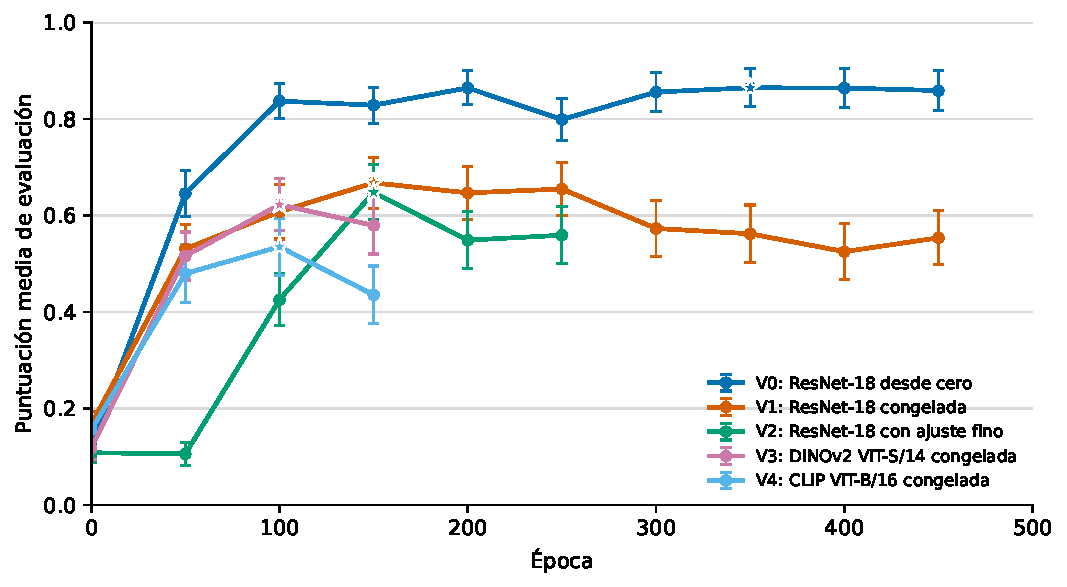
\includegraphics[width=0.92\textwidth]{img/evolucion_puntuacion_prueba.pdf}
  \caption{Evoluci\'on de la puntuaci\'on media de evaluaci\'on de las cinco variantes.}
  \label{fig:evolucion-score}
  \fuente{elaboraci\'on propia}
\end{figure}

V0 alcanza \num{0.8370} en la \'epoca \num{100} y permanece cerca de \num{0.86} durante
la mayor parte del entrenamiento posterior. Su m\'aximo, \num{0.8645}, aparece en la
\'epoca \num{350}; la \'ultima evaluaci\'on, en la \num{450}, conserva \num{0.8588}. La
peque\~na diferencia entre ambos valores indica que la selecci\'on del punto de control no
depende de un pico aislado.

V1 mejora hasta \num{0.6676} en la \'epoca \num{150}. Despu\'es oscila brevemente alrededor
de \num{0.65} y desciende hasta \num{0.5536} en la \'ultima evaluaci\'on. Esta reducci\'on
equivale a \num{0.1140} puntos, un \num{17.1}\,\% respecto a su m\'aximo. En consecuencia,
las \num{350} \'epocas restantes no producen un punto de control mejor.

V2 presenta una convergencia m\'as lenta. Su puntuaci\'on permanece alrededor de
\num{0.11} hasta la \'epoca \num{50}, asciende a \num{0.4253} en la \num{100} y alcanza
\num{0.6477} en la \num{150}. Las dos evaluaciones posteriores caen a \num{0.5487} y
\num{0.5590}. Este comportamiento motiva la detenci\'on anticipada, puesto que prolongar
la ejecuci\'on no hab\'ia recuperado el m\'aximo tras \num{100} \'epocas.

V3 progresa de \num{0.1177} a \num{0.6224} entre las \'epocas \num{0} y \num{100}. La
evaluaci\'on de la \'epoca \num{150} desciende a \num{0.5792}, y la ejecuci\'on se detiene
cuatro \'epocas despu\'es. V4 alcanza \num{0.5351} en la \'epoca \num{100} y cae a
\num{0.4353} en la \num{150}, antes de completar las \num{200} \'epocas asignadas.

La comparaci\'on de los mejores puntos de control sit\'ua V0 por encima de las dem\'as
variantes. Los m\'argenes abarcan desde \num{0.197} frente a V1 hasta \num{0.329} frente a
V4. La \cref{tab:contrastes} relaciona las diez diferencias con su dispersi\'on entre
episodios y con el contraste de Wilcoxon.

\begin{table}[htbp]
  \centering
  \caption{Diferencias pareadas entre los puntos de control seleccionados.}
  \label{tab:contrastes}
  \small
  \scriptsize
  \begin{tabular}{lcccc}
    \toprule
    Comparaci\'on & Diferencia media & IC \SI{95}{\percent} & $p$ & $p_{\mathrm{Holm}}$ \\
    \midrule
    V0 frente a V1 & \num{0.197} & {[\num{0.091};\,\num{0.303}]} & \num{0.0004} & \num{0.0030} \\
    V0 frente a V2 & \num{0.217} & {[\num{0.102};\,\num{0.332}]} & \num{0.0001} & \num{0.0009} \\
    V0 frente a V3 & \num{0.242} & {[\num{0.122};\,\num{0.362}]} & \num{0.0003} & \num{0.0026} \\
    V0 frente a V4 & \num{0.329} & {[\num{0.208};\,\num{0.451}]} & \num{0.000003} & \num{0.000030} \\
    V1 frente a V2 & \num{0.020} & {[\num{-0.093};\,\num{0.133}]} & \num{0.82} & \num{1.00} \\
    V1 frente a V3 & \num{0.045} & {[\num{-0.089};\,\num{0.179}]} & \num{0.46} & \num{1.00} \\
    V1 frente a V4 & \num{0.132} & {[\num{0.018};\,\num{0.247}]} & \num{0.0084} & \num{0.0501} \\
    V2 frente a V3 & \num{0.025} & {[\num{-0.101};\,\num{0.152}]} & \num{0.54} & \num{1.00} \\
    V2 frente a V4 & \num{0.113} & {[\num{-0.034};\,\num{0.259}]} & \num{0.10} & \num{0.5154} \\
    V3 frente a V4 & \num{0.087} & {[\num{-0.027};\,\num{0.201}]} & \num{0.14} & \num{0.5532} \\
    \bottomrule
  \end{tabular}
  \notatabla{Diferencias calculadas sobre los \num{50} episodios comunes. La prueba de
    Wilcoxon emplea la aproximaci\'on normal y los diez valores $p$ se ajustan mediante el
    procedimiento de Holm. Los intervalos no incorporan este ajuste.}
  \fuente{elaboraci\'on propia}
\end{table}

Las cuatro diferencias entre V0 y las variantes preentrenadas excluyen el cero y conservan
significaci\'on tras el ajuste de Holm. Entre las variantes preentrenadas, solo V1 frente a
V4 alcanza significaci\'on sin corregir, con $p = \num{0.0084}$. El ajuste eleva ese valor
a \num{0.0501}, por lo que ning\'un contraste interno supera el umbral familiar del
\SI{5}{\percent}. Estos resultados no cuantifican la variabilidad entre semillas de
entrenamiento, cuesti\'on que se retoma en el \cref{sec:limitaciones}.

\section{Ajuste y generalizaci\'on}
\label{sec:ajuste-resultados}

La puntuaci\'on de la tarea debe interpretarse junto con las p\'erdidas del modelo. La
\cref{fig:evolucion-perdidas} muestra los valores agregados al final de cada \'epoca
completa. La escala logar\'itmica permite observar simult\'aneamente la fase inicial y los
cambios de menor magnitud al final del entrenamiento.

\begin{figure}[htbp]
  \centering
  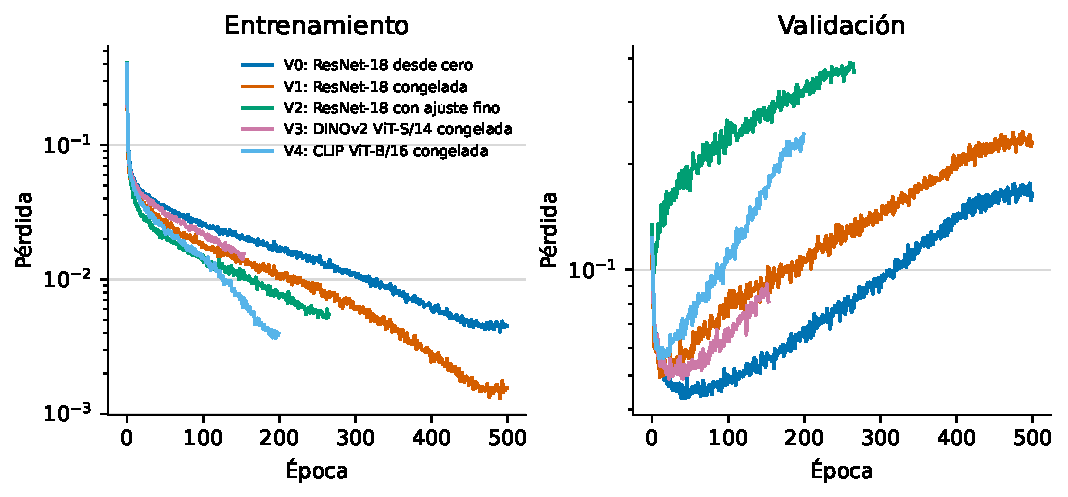
\includegraphics[width=0.95\textwidth]{img/evolucion_perdidas.pdf}
  \caption{Evoluci\'on de las p\'erdidas de entrenamiento y validaci\'on.}
  \label{fig:evolucion-perdidas}
  \fuente{elaboraci\'on propia}
\end{figure}

Las cinco variantes reducen de forma sostenida la p\'erdida de entrenamiento. Sin embargo,
la p\'erdida de validaci\'on vuelve a crecer despu\'es de las primeras \'epocas. El patr\'on
es especialmente claro en V1: entre las \'epocas \num{150} y \num{450}, la p\'erdida de
entrenamiento baja de \num{0.0145} a \num{0.00166}, mientras que la de validaci\'on sube
de \num{0.0869} a \num{0.2247} y la puntuaci\'on de evaluaci\'on disminuye.

V2 muestra la misma divergencia. Entre las \'epocas \num{150} y \num{250}, su p\'erdida de
entrenamiento pasa de \num{0.0115} a \num{0.00587}, la de validaci\'on aumenta de
\num{0.277} a \num{0.380} y la puntuaci\'on pierde \num{0.089} puntos. Ambos casos son
compatibles con sobreajuste. V0 tambi\'en incrementa su p\'erdida de validaci\'on, pero su
puntuaci\'on permanece estable; por tanto, la p\'erdida de predicci\'on del ruido no act\'ua
como sustituto directo del rendimiento en bucle cerrado.

V3 y V4 reproducen esa divergencia. Entre las \'epocas \num{100} y \num{150}, la p\'erdida
de entrenamiento de V3 baja de \num{0.0218} a \num{0.0155}, mientras la de validaci\'on
sube de \num{0.0681} a \num{0.0865}. En V4, las mismas magnitudes pasan de \num{0.0143} a
\num{0.00741} y de \num{0.110} a \num{0.171}. Ambas puntuaciones disminuyen a la vez.

El error cuadr\'atico medio de la acci\'on refuerza esa distinci\'on. En los puntos de
control seleccionados vale \num{116.17} para V0, \num{147.31} para V1, \num{42.86} para
V2, \num{314.78} para V3 y \num{94.93} para V4. V2 obtiene el menor error, pero no la
mejor puntuaci\'on. La precisi\'on sobre acciones registradas y el control en bucle cerrado
miden, por tanto, propiedades diferentes.

\section{Coste computacional}
\label{sec:coste-resultados}

Los tiempos recogidos en la \cref{tab:coste} muestran diferencias amplias. El bucle de V0
requiere \SI{1.6}{\minute} por \'epoca, frente a \SI{5.3}{\minute} en V1,
\SI{14.7}{\minute} en V2, \SI{2.3}{\minute} en V3 y \SI{4.0}{\minute} en V4. Estos valores
multiplican el coste de la l\'inea base por factores entre \num{1.5} y \num{9.5}.

V2 a\~nade la retropropagaci\'on a trav\'es del codificador y presenta el mayor coste por
\'epoca. V4 duplica las actualizaciones debido a su lote de \num{32} muestras. V3 muestra,
sin embargo, que operar a \num{224} p\'ixeles no determina por s\'i solo el tiempo: su
codificador congelado queda m\'as cerca de V0 que de V1.

Conviene no confundir ese coste unitario con el tiempo total. V2 acumula \SI{84.9}{\hour}
frente a las \SI{96.5}{\hour} de V1 pese a ser la variante m\'as cara por \'epoca, porque
se detuvo antes. V3 solo suma \SI{10.9}{\hour} por la misma raz\'on. La comparaci\'on v\'alida
entre variantes es el tiempo por \'epoca; el total de \SI{237.1}{\hour} describe el
experimento ejecutado con presupuestos distintos.

\section{Comprobaci\'on cualitativa}
\label{sec:resultados-cualitativos}

Los cuadernos de inferencia permiten inspeccionar trayectorias individuales de los mejores
puntos de control. La \cref{fig:inferencia-v1-v2} compara V1 y V2 desde la misma condici\'on
inicial, generada con la semilla \num{10049}. Cada panel muestra el estado inicial, el
estado final y la puntuaci\'on instant\'anea durante el episodio.

\begin{figure}[!t]
  \centering
  \begin{subfigure}{0.98\textwidth}
    \centering
    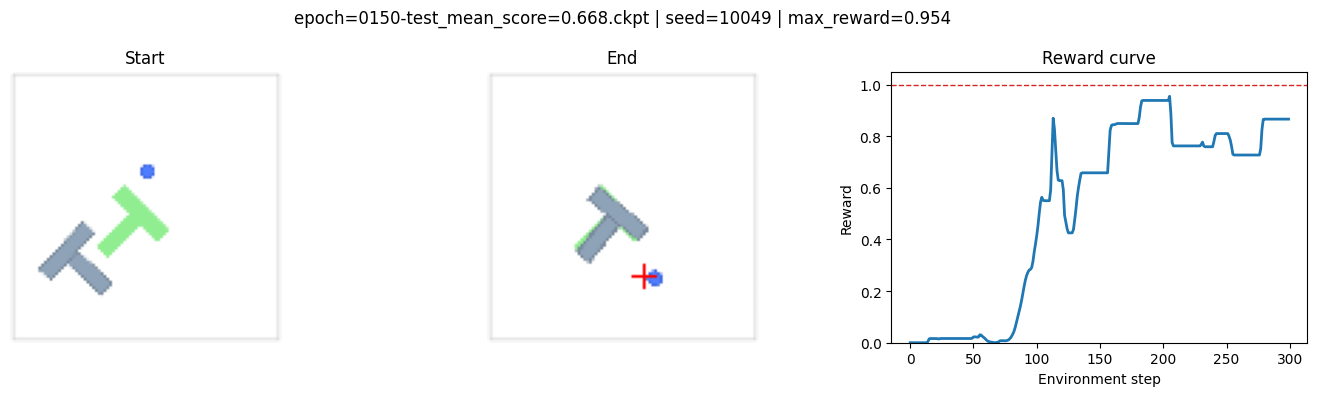
\includegraphics[width=\linewidth]{img/inferencia_v1.png}
    \caption{V1, ResNet-18 preentrenada y congelada.}
    \label{fig:inferencia-v1}
  \end{subfigure}

  \vspace{6pt}

  \begin{subfigure}{0.98\textwidth}
    \centering
    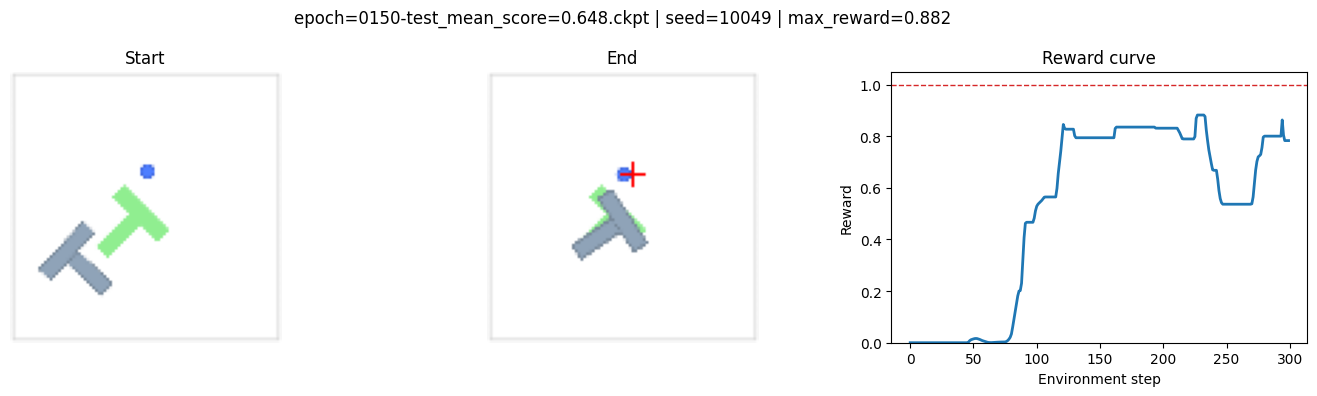
\includegraphics[width=\linewidth]{img/inferencia_v2.png}
    \caption{V2, ResNet-18 preentrenada con ajuste fino.}
    \label{fig:inferencia-v2}
  \end{subfigure}
  \caption{Inferencia de V1 y V2 sobre una condici\'on inicial compartida.}
  \label{fig:inferencia-v1-v2}
  \fuente{elaboraci\'on propia}
\end{figure}

V1 alcanza una puntuaci\'on m\'axima de \num{0.9544}, frente a \num{0.8818} en V2. Ninguna
de las dos trayectorias llega al umbral unitario de \'exito, aunque V1 consigue una
superposici\'on mayor. V0 s\'i alcanza \num{1.0} en su cuaderno, pero parte de la semilla
\num{10000}; por ese motivo, su trayectoria no se incorpora a la comparaci\'on visual.

Estas demostraciones no sustituyen la evaluaci\'on cuantitativa. Sus semillas quedan fuera
del intervalo oficial \num{100000}--\num{100049} y cada imagen representa un solo episodio.
Adem\'as, la puntuaci\'on mostrada es el m\'aximo temporal, no el valor del estado final.
Su funci\'on es ilustrar el comportamiento que origina la m\'etrica, no estimar el
rendimiento medio.

\section{Contraste de las hip\'otesis}
\label{sec:contraste-hipotesis}

La primera hip\'otesis planteaba que el preentrenamiento aportar\'ia representaciones m\'as
\'utiles que el entrenamiento desde cero. Los resultados no la respaldan: V0 supera entre
\num{0.197} y \num{0.329} puntos a las cuatro variantes preentrenadas. Todas las
diferencias conservan significaci\'on tras el ajuste de Holm.

La segunda hip\'otesis propon\'ia una ventaja del ajuste fino sobre la congelaci\'on. Tampoco
queda respaldada, ya que V1 obtiene \num{0.668} y V2 \num{0.648}. La diferencia de
\num{0.020} no alcanza significaci\'on ($p = \num{0.82}$) y su intervalo de confianza,
{[\num{-0.093};\,\num{0.133}]}, contiene el cero. En consecuencia, tampoco cabe afirmar la
superioridad de la congelaci\'on: lo que descarta la evidencia es una mejora observable del
ajuste fino en esta ejecuci\'on.

La tercera hip\'otesis propon\'ia que los transformadores alcanzar\'ian un rendimiento
comparable al de las redes convolucionales con mayor coste de inferencia. V3 y V4 quedan
por debajo de V0, pero no se distinguen de V1 y V2 tras la correcci\'on familiar. Por tanto,
los datos no muestran una ventaja de rendimiento propia de la arquitectura ViT. La parte
relativa a inferencia no puede contrastarse porque no se midi\'o su latencia bajo un
protocolo com\'un.

\section{Limitaciones}
\label{sec:limitaciones}

La primera limitaci\'on es la desigualdad del presupuesto de \'epocas. V0 y V1 acumulan
diez evaluaciones, V2 seis, y V3 y V4 solo cuatro. V3 se interrumpi\'o tras \num{155}
\'epocas de las \num{300} previstas, de modo que no puede descartarse una recuperaci\'on
posterior. La comparaci\'on corresponde a los mejores puntos observados dentro de esos
presupuestos, no a curvas con igual horizonte.

La segunda limitaci\'on es el uso de una sola semilla de entrenamiento. Los intervalos y
los contrastes de la \cref{tab:contrastes} cuantifican la dispersi\'on debida a las
condiciones iniciales del simulador, ya que los \num{50} episodios son condiciones
distintas evaluadas con el mismo modelo. No cuantifican, en cambio, la variabilidad entre
ejecuciones de entrenamiento, puesto que cada variante se ha ajustado una sola vez. Una
r\'eplica con otra semilla podr\'ia desplazar las curvas, y esa incertidumbre queda fuera
de las cifras reportadas.

La tercera afecta a la selecci\'on del modelo. Las \num{50} condiciones reservadas se
eval\'uan peri\'odicamente y determinan qu\'e punto de control se conserva, de modo que
act\'uan como conjunto de selecci\'on y no como evaluaci\'on final independiente, tal como
precisa el \cref{sec:metricas}. El m\'aximo reportado presenta por ello un sesgo optimista,
que la media de las tres \'ultimas evaluaciones ayuda a acotar. Cerrar el problema
exigir\'ia evaluar los puntos de control seleccionados sobre un bloque de semillas disjunto
del empleado en la selecci\'on, medida que no se ha ejecutado y que se propone en el
\cref{sec:trabajo-futuro}.

Por \'ultimo, la evaluaci\'on cada \num{50} \'epocas ofrece una visi\'on discreta de la
trayectoria y puede omitir m\'aximos intermedios. V2 a\~nade una reanudaci\'on, y solo su
tiempo acumulado requiere extrapolaci\'on parcial. Estas restricciones aconsejan
interpretar las cifras como evidencia del experimento realizado, no como una ordenaci\'on
universal de los codificadores.

\chapter{Conclusiones}
\label{cap:conclusiones}

Este cap\'itulo interpreta los resultados del \cref{cap:resultados} a la luz de los
objetivos y las hip\'otesis enunciados en los cap\'itulos anteriores. En primer lugar,
formula una conclusi\'on por cada objetivo espec\'ifico y precisa qu\'e permiten afirmar
los datos. A continuaci\'on, expone las l\'ineas de continuaci\'on abiertas por el
estudio.

Conviene advertir de entrada que el estudio es parcial. Las variantes V3 y V4 siguen en
ejecuci\'on, de modo que las conclusiones sobre el rendimiento se apoyan en las tres
variantes convolucionales completadas.

\section{Conclusiones del trabajo}
\label{sec:conclusiones}

\divisionmenor{Sobre la implementaci\'on de las variantes}

El primer objetivo espec\'ifico se cumple en su totalidad en cuanto a la implementaci\'on.
Las cinco variantes del codificador visual funcionan dentro de la misma
\textit{Diffusion Policy}, entregan un vector de condicionamiento de id\'entica
dimensi\'on y comparten red generativa, hiperpar\'ametros y protocolo de evaluaci\'on. La
comparaci\'on entre ellas queda as\'i acotada al bloque visual.

En cambio, la ejecuci\'on solo se ha completado para tres de las cinco variantes. Por
tanto, el trabajo responde ya a la segunda pregunta planteada en el \cref{sec:problema},
la relativa a la estrategia de entrenamiento, mientras que la primera, la relativa a la
arquitectura del codificador, queda abierta hasta disponer de V3 y V4.

\divisionmenor{Sobre el rendimiento de las variantes}

La conclusi\'on principal del trabajo contradice la hip\'otesis de partida: el bloque
formado por el codificador preentrenado sobre ImageNet y su cadena de preprocesado no
mejora el rendimiento en Push-T, sino que lo degrada de forma sustancial. La l\'inea base
entrenada desde cero alcanza una puntuaci\'on media de evaluaci\'on de \num{0.864}, frente
a \num{0.668} de la variante congelada y \num{0.648} de la ajustada. Las ca\'idas equivalen
al \SI{23}{\percent} y al \SI{25}{\percent} del valor de referencia. Ambas diferencias
superan la dispersi\'on entre episodios: sus intervalos de confianza al \SI{95}{\percent},
{[\num{0.091};\,\num{0.303}]} y {[\num{0.102};\,\num{0.332}]}, excluyen el cero, con
$p = \num{0.0004}$ y $p = \num{0.0001}$ en la prueba de los rangos con signo.

Asimismo, la segunda hip\'otesis tampoco se sostiene. El ajuste fino del codificador
preentrenado no supera a su congelaci\'on, puesto que V2 se queda \num{0.020} por debajo de
V1. Esa diferencia no alcanza significaci\'on ($p = \num{0.82}$) y su intervalo contiene el
cero, de modo que la conclusi\'on correcta no es que la congelaci\'on sea mejor, sino que
actualizar los pesos preentrenados no aporta ninguna ventaja medible. La incertidumbre
entre semillas de entrenamiento, no cuantificada, se suma a esa indeterminaci\'on.

El ajuste fino s\'i altera, en cambio, la din\'amica del entrenamiento, y siempre a peor.
V2 permanece estancada alrededor de \num{0.11} hasta la \'epoca \num{50}, cuando V0 y V1
ya rebasan \num{0.53}. Adem\'as, sobreajusta antes y con mayor intensidad: en la \'epoca
\num{250} su p\'erdida de validaci\'on alcanza \num{0.380}, frente a \num{0.120} de V1 y
\num{0.077} de V0. En conjunto, la actualizaci\'on de los pesos degrada la
representaci\'on de partida sin construir otra m\'as \'util con las demostraciones
disponibles.

Una explicaci\'on plausible atiende a la distancia entre dominios. Las observaciones de
Push-T son im\'agenes sint\'eticas de fondo uniforme, sin textura y con pocas formas,
mientras que las caracter\'isticas aprendidas sobre ImageNet codifican textura y categor\'ia
de objeto \cite{deng2009imagenet}. Esa informaci\'on resulta poco pertinente en una tarea
definida por la posici\'on relativa de dos figuras geom\'etricas. La observaci\'on es
coherente con dos antecedentes: R3M, preentrenado sobre v\'ideo, tampoco supera al
codificador entrenado de extremo a extremo en Push-T \cite{nair2022r3m},
\cite{chi2025diffusion}, y el estudio con DINOv3 concluye que la ventaja del
preentrenamiento depende de la tarea y de la estrategia de adaptaci\'on
\cite{egbe2025dinov3dp}.

La atribuci\'on causal exige, en cambio, una precisi\'on que recorre todo este apartado.
V0 difiere de V1 y V2 en cuatro factores a la vez, ya que el preprocesado viaja con los
pesos: la inicializaci\'on, la resoluci\'on de entrada (\num{96} frente a \num{224}
p\'ixeles), el recorte aleatorio, que solo aplica la l\'inea base, y la agregaci\'on
espacial a la salida del codificador. Sobre este \'ultimo conviene detenerse: V0 conserva
la localizaci\'on de las activaciones mediante un \textit{spatial softmax}
\cite{levine2016visuomotor}, mientras que las variantes preentrenadas entregan un
descriptor global. En una tarea definida por posiciones relativas, esa p\'erdida de
informaci\'on geom\'etrica puede resultar tan explicativa como la propia inicializaci\'on.

Las conclusiones anteriores se refieren, por tanto, al codificador junto con su cadena de
preprocesado, entendidos como un bloque, y no a la inicializaci\'on aislada. Separar los
cuatro efectos requiere entrenamientos adicionales, descritos en el
\cref{sec:trabajo-futuro}.

\divisionmenor{Sobre el coste computacional}

La l\'inea base no solo obtiene la mejor puntuaci\'on, sino que adem\'as es la m\'as
barata. Cada \'epoca de V0 ocupa \SI{1.5}{\minute}, frente a \SI{5.3}{\minute} de V1 y
\SI{14.7}{\minute} de V2, esto es, factores de \num{3.5} y \num{9.8}. En tiempo total, V0
consume \SI{17.4}{\hour} de GPU frente a \SI{96.5}{\hour} de V1 y \SI{84.9}{\hour} de V2,
y esta \'ultima cifra resulta menor solo porque su ejecuci\'on se detuvo antes. Las
variantes preentrenadas son, por tanto, simult\'aneamente peores y m\'as costosas,
combinaci\'on que no deja margen para un compromiso entre rendimiento y coste.

Ese sobrecoste no procede del n\'umero de par\'ametros entrenables. V1 congela el
codificador y entrena \num{277} millones de par\'ametros frente a los \num{288} millones de
V0, una reducci\'on del \SI{4}{\percent}, y aun as\'i cada \'epoca le cuesta tres veces y
media m\'as. El factor
determinante es la resoluci\'on de entrada, dado que una imagen de \num{224} p\'ixeles
contiene \num{5.4} veces m\'as p\'ixeles que una de \num{96}. De ah\'i se sigue una
conclusi\'on de alcance pr\'actico: congelar un codificador no abarata el entrenamiento
cuando obliga a ampliar la imagen de entrada.

\divisionmenor{Respuesta al objetivo general}

En conjunto, y para la configuraci\'on estudiada, la respuesta al objetivo general resulta
inequ\'ivoca en su parte convolucional. Con \num{206} demostraciones de Push-T, una
ResNet-18 entrenada de extremo a extremo a resoluci\'on nativa domina en rendimiento y en
coste a las dos alternativas preentrenadas sobre ImageNet. Ning\'un dato del estudio
respalda sustituirla por ellas.

Queda por determinar si esa conclusi\'on se extiende a los codificadores preentrenados con
objetivos distintos de la clasificaci\'on supervisada. Las representaciones
autosupervisadas de DINOv2 \cite{oquab2024dinov2} y las multimodales de CLIP
\cite{radford2021clip} podr\'ian conservar informaci\'on espacial m\'as pertinente para la
tarea. Los entrenamientos de V3 y V4 se encuentran en curso y decidir\'an ese punto.
[PENDIENTE: resultados de V3 y V4]

\section{Trabajo futuro}
\label{sec:trabajo-futuro}

Del estudio se derivan seis l\'ineas de continuaci\'on, ordenadas por su capacidad para
afianzar o corregir las conclusiones anteriores.

En primer lugar, completar las variantes V3 y V4. Ambas discriminan entre dos lecturas de
la conclusi\'on principal: que el problema resida en la supervisi\'on de ImageNet o que
afecte a todo codificador preentrenado fuera del dominio rob\'otico.

En segundo lugar, aislar los cuatro factores confundidos entre la l\'inea base y las
variantes preentrenadas. Un entrenamiento adicional de ResNet-18 desde cero a \num{224}
p\'ixeles y sin recorte aleatorio separa el efecto de la inicializaci\'on del efecto del
preprocesado. Su coste por \'epoca coincide con el de V2, del orden de
\SI{15}{\minute}, puesto que el codificador se actualiza en ambos casos y la resoluci\'on
de entrada es la misma; bajo el criterio de parada, el total se sit\'ua en torno a las
\SI{85}{\hour}. Una segunda ejecuci\'on desde cero a \num{96} p\'ixeles y sin recorte
aleatorio aislar\'ia el efecto del aumento de datos por unas \SI{17}{\hour}, coste
equivalente al de V0.

En tercer lugar, repetir las variantes seleccionadas con las semillas \num{43} y \num{44}.
Los contrastes del \cref{cap:resultados} cubren la dispersi\'on entre condiciones iniciales,
pero no la variabilidad entre ejecuciones de entrenamiento; solo la r\'eplica permite
estimarla, limitaci\'on declarada desde el \cref{sec:alcance} y cuantificada en el
\cref{sec:coste}.

En cuarto lugar, evaluar los puntos de control seleccionados sobre un bloque de semillas de
entorno disjunto del empleado para seleccionarlos. Ese paso convertir\'ia la medida actual,
que act\'ua como puntuaci\'on de selecci\'on, en una evaluaci\'on final independiente, y su
coste se reduce a tres ejecuciones de inferencia.

En quinto lugar, examinar la agregaci\'on espacial a la salida de los codificadores
preentrenados. La l\'inea base conserva la localizaci\'on de las activaciones mediante un
\textit{spatial softmax} \cite{levine2016visuomotor}, mientras que las variantes
preentrenadas entregan un descriptor global. Cabe evaluar si una agregaci\'on que preserve
la geometr\'ia recupera parte de la diferencia observada.

Por \'ultimo, extender el protocolo a otras tareas y a un robot f\'isico. Push-T aporta un
banco de pruebas controlado, pero sus im\'agenes sint\'eticas son precisamente el escenario
menos favorable para un codificador preentrenado sobre fotograf\'ias naturales. La
conclusi\'on podr\'ia invertirse en observaciones reales, extremo que este trabajo no puede
resolver.

\chapter{Presupuesto}
\label{cap:presupuesto}

Este cap\'itulo cuantifica el coste de ejecuci\'on del proyecto. El presupuesto recoge
cuatro partidas: material fungible y suministros, amortizaci\'on de los equipos, licencias
de software y mano de obra. A ellas se a\~naden unos costes indirectos y, con todo, se
obtiene el importe total.

Tres criterios de imputaci\'on gobiernan las cifras que siguen. En primer lugar, el
periodo imputado abarca siete meses, de marzo a septiembre de 2026, que comprenden
desde la revisi\'on bibliogr\'afica hasta la entrega de la memoria. En segundo lugar, los
equipos se amortizan de forma lineal y se imputa la fracci\'on correspondiente a esos
siete meses, con independencia de su uso efectivo dentro de cada jornada. En tercer lugar,
los importes se expresan sin impuestos indirectos, puesto que el trabajo se desarrolla en
el \'ambito acad\'emico y no da lugar a facturaci\'on.

\section{Material fungible y suministros}
\label{sec:fungible}

El proyecto es de naturaleza computacional, de modo que apenas consume material f\'isico.
La \'unica partida relevante es la energ\'ia el\'ectrica, dominada por los entrenamientos
desatendidos. Seg\'un el \cref{sec:coste}, estos ocuparon \SI{237.1}{\hour} de c\'omputo;
con un consumo aproximado de \SI{150}{\watt} bajo carga, suman unos \num{36}
kilovatios-hora. El resto de la dedicaci\'on a\~nade otros \num{24} kilovatios-hora, con el
equipo en r\'egimen de trabajo ordinario. El precio de \num{0.15}~\texteuro{} por
kilovatio-hora es una tarifa convencional de imputaci\'on adoptada para el proyecto, no un
precio contratado. La \cref{tab:fungible} recoge ambos conceptos.

\begin{table}[htbp]
  \centering
  \caption{Presupuesto de material fungible y suministros.}
  \label{tab:fungible}
  \small
  \begin{tabular}{lrrr}
    \toprule
    Concepto & Cantidad & Coste unitario (\texteuro) & Total (\texteuro) \\
    \midrule
    Energ\'ia el\'ectrica (kWh)        & \num{60} & \num{0.15} & \num{9.00} \\
    Material de oficina e impresi\'on  & \num{1}  & \num{45.00} & \num{45.00} \\
    \midrule
    \textbf{Total} & & & \textbf{\num{54.00}} \\
    \bottomrule
  \end{tabular}
  \notatabla{Se adopta un precio de \num{0.15} \texteuro/kWh, valor de referencia para el
    suministro dom\'estico durante el periodo imputado.}
  \fuente{elaboraci\'on propia}
\end{table}

\section{Amortizaci\'on de los equipos}
\label{sec:equipos}

El proyecto se ejecuta sobre un \'unico equipo, descrito en el \cref{sec:entorno}. Dado
que su vida \'util excede la duraci\'on del trabajo, no se imputa el precio de
adquisici\'on sino la amortizaci\'on correspondiente al periodo de uso, seg\'un la
\cref{eq:amortizacion}.

\begin{equation}
  A = C \cdot \frac{t}{V}
  \label{eq:amortizacion}
\end{equation}

En la \cref{eq:amortizacion}, $A$ es el importe imputado, $C$ el precio de adquisici\'on,
$t$ el periodo de uso y $V$ la vida \'util, ambos expresados en meses. Se aplica
amortizaci\'on lineal y sin valor residual, criterio habitual para equipos de proceso de
informaci\'on. La \cref{tab:equipos} detalla el resultado para cada elemento.

\begin{table}[htbp]
  \centering
  \caption{Amortizaci\'on de los equipos imputada al proyecto.}
  \label{tab:equipos}
  \small
  \begin{tabular}{lrrrr}
    \toprule
    Equipo & Precio (\texteuro) & Vida \'util (a\~nos) & Uso (meses) &
      Imputaci\'on (\texteuro) \\
    \midrule
    Port\'atil con GPU dedicada & \num{1800.00} & \num{4} & \num{7} & \num{262.50} \\
    Monitor externo                & \num{180.00}  & \num{5} & \num{7} & \num{21.00} \\
    Unidad externa de respaldo     & \num{60.00}   & \num{3} & \num{7} & \num{11.67} \\
    \midrule
    \textbf{Total} & & & & \textbf{\num{295.17}} \\
    \bottomrule
  \end{tabular}
  \fuente{elaboraci\'on propia}
\end{table}

Conviene se\~nalar que la unidad de procesamiento gr\'afico condiciona el dise\~no
experimental, seg\'un se argument\'o en el \cref{sec:entorno}, pero apenas condiciona el
presupuesto. Su amortizaci\'on forma parte de los \num{262.50} \texteuro{} imputados al
port\'atil, importe menor que el coste de dos jornadas de trabajo.

\section{Licencias de software}
\label{sec:software}

Todas las herramientas empleadas son de c\'odigo abierto o de uso gratuito, de modo que
esta partida asciende a \num{0.00} \texteuro. La \cref{tab:componentes} enumera la pila de
software: Python, PyTorch, torchvision, timm, diffusers, robomimic, Hydra y Zarr se
distribuyen bajo licencias libres. A ellas se suman la distribuci\'on Ubuntu, el sistema
de composici\'on \TeX{} Live y el control de versiones Git, tambi\'en libres. La licencia de
Windows 11 viene incluida en el precio del port\'atil y queda, por tanto, recogida en el
\cref{sec:equipos}.

\section{Mano de obra}
\label{sec:mano-de-obra}

La mano de obra distingue dos perfiles. El autor asume la implementaci\'on, la
ejecuci\'on, el an\'alisis y la redacci\'on, con el coste horario de un ingeniero de datos
junior. El director asume la definici\'on del alcance, el seguimiento peri\'odico y la
revisi\'on de la memoria, con el coste horario de un investigador s\'enior. Ambos importes
corresponden al coste bruto para la entidad, incluidas las cargas sociales. Conviene declarar
su origen: son tarifas convencionales de imputaci\'on adoptadas para el proyecto, de un orden
habitual para esos dos perfiles, y no proceden de una tabla salarial ni de una fuente
retributiva concreta. El
presupuesto es, en consecuencia, una estimaci\'on del orden de magnitud del coste y no una
oferta; la mano de obra domina el total, de modo que cualquier revisi\'on de esas tarifas se
traslada casi \'integramente a la cifra final.

La \cref{tab:horas} desglosa la dedicaci\'on del autor por fases. El reparto refleja el
peso real de cada actividad: la preparaci\'on del entorno de c\'omputo result\'o m\'as
costosa de lo previsto, mientras que la ejecuci\'on de los entrenamientos, aunque ocup\'o
m\'as de \num{237} horas de m\'aquina, exigi\'o poca intervenci\'on por tratarse de procesos
desatendidos.

\begin{table}[htbp]
  \centering
  \caption{Dedicaci\'on del autor por fases del proyecto.}
  \label{tab:horas}
  \small
  \begin{tabular}{lr}
    \toprule
    Fase & Horas \\
    \midrule
    Revisi\'on bibliogr\'afica y estado del arte          & \num{70} \\
    Preparaci\'on del entorno de c\'omputo                & \num{55} \\
    Implementaci\'on de las variantes del codificador     & \num{90} \\
    Ejecuci\'on y supervisi\'on de los entrenamientos     & \num{60} \\
    An\'alisis de resultados y comprobaci\'on cualitativa & \num{65} \\
    Redacci\'on de la memoria                             & \num{110} \\
    \midrule
    \textbf{Total} & \textbf{\num{450}} \\
    \bottomrule
  \end{tabular}
  \fuente{elaboraci\'on propia}
\end{table}

La dedicaci\'on del director se estima en \num{40} horas: unas \num{20} reuniones de
seguimiento de una hora, repartidas a lo largo de los siete meses, y otras \num{20} horas
de revisi\'on de los borradores. La \cref{tab:mano-de-obra} aplica los costes horarios a
ambos perfiles.

\begin{table}[htbp]
  \centering
  \caption{Presupuesto de mano de obra.}
  \label{tab:mano-de-obra}
  \small
  \begin{tabular}{lrrr}
    \toprule
    Perfil & Horas & Coste horario (\texteuro) & Total (\texteuro) \\
    \midrule
    Ingeniero de datos junior (autor) & \num{450} & \num{30.00} & \num{13500.00} \\
    Investigador s\'enior (director)  & \num{40}  & \num{60.00} & \num{2400.00} \\
    \midrule
    \textbf{Total} & \textbf{\num{490}} & & \textbf{\num{15900.00}} \\
    \bottomrule
  \end{tabular}
  \fuente{elaboraci\'on propia}
\end{table}

\section{Resumen del presupuesto}
\label{sec:resumen-presupuesto}

La \cref{tab:resumen-presupuesto} agrega las cuatro partidas anteriores y a\~nade unos
costes indirectos del \SI{15}{\percent} sobre el subtotal, porcentaje que cubre espacio de
trabajo, conectividad y servicios generales no imputables a un concepto concreto.

\begin{table}[htbp]
  \centering
  \caption{Resumen del presupuesto.}
  \label{tab:resumen-presupuesto}
  \small
  \begin{tabular}{lr}
    \toprule
    Partida & Importe (\texteuro) \\
    \midrule
    Material fungible y suministros & \num{54.00} \\
    Amortizaci\'on de equipos       & \num{295.17} \\
    Licencias de software           & \num{0.00} \\
    Mano de obra                    & \num{15900.00} \\
    \midrule
    Subtotal                        & \num{16249.17} \\
    Costes indirectos (\SI{15}{\percent}) & \num{2437.38} \\
    \midrule
    \textbf{Total}                  & \textbf{\num{18686.55}} \\
    \bottomrule
  \end{tabular}
  \fuente{elaboraci\'on propia}
\end{table}

El coste total del proyecto asciende, por tanto, a \num{18686.55} \texteuro. La
distribuci\'on entre partidas resulta muy desigual: la mano de obra representa el
\SI{85}{\percent} del total, mientras que los equipos apenas alcanzan el
\SI{1.6}{\percent}. Esa asimetr\'ia es caracter\'istica de un proyecto de investigaci\'on
computacional ejecutado sobre hardware propio.

De ah\'i se sigue una consideraci\'on econ\'omica sobre el dise\~no experimental. Las
limitaciones descritas en el \cref{sec:coste} no proceden del presupuesto, sino del tiempo
de calendario: ampliar el estudio a tres semillas por variante multiplicar\'ia por tres el
c\'omputo sin apenas alterar el coste, ya que la amortizaci\'on y la energ\'ia son
partidas menores. El factor limitante es que esas horas de m\'aquina deben transcurrir
dentro del plazo del proyecto, no lo que cuestan.


% ============================ REFERENCIAS ===================================
% Lista IEEE unica, numerada por orden de aparicion. Solo obras citadas en el
% texto: el sistema IEEE exige correspondencia univoca entre cita y entrada.
% La antigua lista separada "Bibliografia" se retiro; sus dos entradas propias
% (monografia y repositorio) pasaron a bib/referencias.bib y se citan en el
% cuerpo, en sec:entorno.
\cleardoublepage
\phantomsection
\addcontentsline{toc}{chapter}{Referencias}
\renewcommand{\bibname}{Referencias}
\bibliographystyle{bst/IEEEtran}
\bibliography{bib/referencias}

% Sin anexos: el material de apoyo (configuraciones efectivas, registros,
% guiones de analisis y protocolo) reside en el repositorio del trabajo, que se
% cita formalmente. Los identificadores, huellas y configuraciones necesarios
% para reproducir el experimento estan en sec:entorno y sec:protocolo.

\end{document}
